\documentclass[12pt,a4paper]{report}

% =============================================================================
% CORE PACKAGES
% =============================================================================
\usepackage[utf8]{inputenc}
\usepackage[T1]{fontenc}
\usepackage{mathptmx} % Times New Roman equivalent font
\usepackage{amsmath,amssymb}
\usepackage{graphicx}
\usepackage{booktabs}
\usepackage{tabularx}
\usepackage{colortbl}
\usepackage{xcolor}
\usepackage{listings}
\usepackage{setspace}
\usepackage[left=1.25in,right=1.0in,top=1.0in,bottom=1.0in,headheight=15pt]{geometry}
\usepackage{fancyhdr}
\usepackage{titlesec}
\usepackage{tocloft}
\usepackage{enumitem}
\usepackage{microtype}
\usepackage[hidelinks,colorlinks=true,linkcolor=black,citecolor=blue!70!black,urlcolor=blue!70!black]{hyperref}

% =============================================================================
% FORMATTING AND STYLING CONFIGURATION
% =============================================================================
\setstretch{1.3} % 1.3 to 1.5 line spacing for academic clarity

% Table of Contents dots and spacing
\renewcommand{\cftchapleader}{\cftdotfill{\cftdotsep}}
\renewcommand{\cftsecleader}{\cftdotfill{\cftdotsep}}
\renewcommand{\cftsubsecleader}{\cftdotfill{\cftdotsep}}
\setlength{\cftbeforechapskip}{6pt}

% Section Heading Formatting
\titleformat{\chapter}[display]
  {\normalfont\Large\bfseries\centering}
  {\MakeUppercase{\chaptertitlename\ \thechapter}}
  {8pt}
  {\LARGE\MakeUppercase}
\titlespacing*{\chapter}{0pt}{-10pt}{20pt}

\titleformat{\section}
  {\normalfont\large\bfseries}{\thesection}{1em}{\MakeUppercase}
\titleformat{\subsection}
  {\normalfont\normalsize\bfseries}{\thesubsection}{1em}{}
\titleformat{\subsubsection}
  {\normalfont\normalsize\bfseries}{\thesubsubsection}{1em}{}

% Header and Footer Setup
\pagestyle{fancy}
\fancyhf{}
\fancyhead[R]{\thepage}
\fancyhead[L]{\small\nouppercase{\leftmark}}
\renewcommand{\headrulewidth}{0.5pt}
\renewcommand{\footrulewidth}{0pt}

% Code Listing Configuration
\definecolor{codegreen}{rgb}{0,0.5,0}
\definecolor{codegray}{rgb}{0.45,0.45,0.45}
\definecolor{codepurple}{rgb}{0.55,0,0.8}
\definecolor{codeback}{rgb}{0.97,0.97,0.98}

\lstdefinestyle{customcode}{
    backgroundcolor=\color{codeback},
    commentstyle=\color{codegreen}\itshape,
    keywordstyle=\color{blue!80!black}\bfseries,
    numberstyle=\tiny\color{codegray},
    stringstyle=\color{codepurple},
    basicstyle=\ttfamily\scriptsize,
    breakatwhitespace=false,
    breaklines=true,
    captionpos=b,
    keepspaces=true,
    numbers=left,
    numbersep=6pt,
    showspaces=false,
    showstringspaces=false,
    showtabs=false,
    tabsize=2,
    frame=single,
    rulecolor=\color{black!20}
}
\lstset{style=customcode}

% =============================================================================
% DOCUMENT COMMENCES
% =============================================================================
\begin{document}

% -----------------------------------------------------------------------------
% TITLE / COVER PAGE
% -----------------------------------------------------------------------------
\begin{titlepage}
\centering
\vspace*{0.5cm}

{\Large \textbf{SRM INSTITUTE OF SCIENCE AND TECHNOLOGY}}\\[0.2cm]
{\small (Deemed to be University under section 3 of UGC Act, 1956)}\\[0.3cm]
{\large \textbf{COLLEGE OF ENGINEERING AND TECHNOLOGY}}\\[0.2cm]
{\large \textbf{DEPARTMENT OF ELECTRONICS AND COMMUNICATION ENGINEERING}}\\[1.2cm]

{\Large \textbf{21ECC402P -- COMPUTER COMMUNICATION AND NETWORK SECURITY}}\\[0.3cm]
{\large \textbf{ACADEMIC YEAR: 2026--2027 (ODD SEMESTER)}}\\[1.2cm]

{\LARGE \textbf{AI-ASSISTED IOT WI-FI NETWORK SECURITY AND ANOMALY DETECTION}}\\[0.5cm]
{\large \textbf{Dual-Detector SOC Architecture with Sample-Gated Isolation Forests and Resilient Edge Persistence}}\\[1.5cm]

{\large \textbf{A PROJECT REPORT}}\\[0.3cm]
{\normalsize \textit{Submitted in partial fulfillment of the requirements for the course evaluation}}\\[1.2cm]

\textbf{SUBMITTED BY:}\\[0.3cm]
\begin{tabular}{ll}
\textbf{B. KARTHIK BABU} & \textbf{(Reg. No. RA2311053010001)} \\
\textbf{MEGHA SARA BAIJU} & \textbf{(Reg. No. RA2311053010002)} \\
\textbf{YEMPARA NEEHARIKA} & \textbf{(Reg. No. RA2311053010003)} \\
\end{tabular}\\[1.5cm]

\textbf{UNDER THE GUIDANCE OF:}\\[0.2cm]
\textbf{S. DIANA EMERALD AASHA}\\[0.1cm]
{\normalsize Assistant Professor, Department of ECE}\\[1.2cm]

{\normalsize SRM Nagar, Kattankulathur -- 603 203, Chengalpattu District, Tamil Nadu, India}\\[0.2cm]
{\normalsize November 2026}

\end{titlepage}

% -----------------------------------------------------------------------------
% FRONT MATTER (ROMAN PAGE NUMBERING)
% -----------------------------------------------------------------------------
\pagenumbering{roman}
\setcounter{page}{2}

% Bonafide Certificate
\chapter*{BONAFIDE CERTIFICATE}
\addcontentsline{toc}{chapter}{BONAFIDE CERTIFICATE}
\thispagestyle{plain}

Certified that this project report titled \textbf{``AI-ASSISTED IOT WI-FI NETWORK SECURITY AND ANOMALY DETECTION''} is the bonafide work of \textbf{B. KARTHIK BABU (RA2311053010001)}, \textbf{MEGHA SARA BAIJU (RA2311053010002)}, and \textbf{YEMPARA NEEHARIKA (RA2311053010003)} who carried out the project work under my supervision for the course \textbf{21ECC402P -- Computer Communication and Network Security} in the Department of Electronics and Communication Engineering, College of Engineering and Technology, SRM Institute of Science and Technology, Kattankulathur during the academic year 2026--2027 (Odd Semester).

\vspace{3.0cm}

\noindent
\begin{tabular}{p{7.5cm}p{7.5cm}}
\textbf{SUPERVISOR} & \textbf{HEAD OF THE DEPARTMENT} \\[0.2cm]
\textbf{S. Diana Emerald Aasha} & \textbf{Dr. Shanthi Prince} \\
Assistant Professor & Professor and Head \\
Department of ECE & Department of ECE \\
SRM Institute of Science and Technology & SRM Institute of Science and Technology \\
Kattankulathur -- 603 203 & Kattankulathur -- 603 203 \\
\end{tabular}

\vspace{2.5cm}
\noindent
Submitted for the project viva-voce examination held on \rule{4cm}{0.4pt} at SRM Institute of Science and Technology, Kattankulathur.

\vspace{1.5cm}
\noindent
\begin{tabular}{p{7.5cm}p{7.5cm}}
\textbf{INTERNAL EXAMINER} & \textbf{EXTERNAL EXAMINER} \\
\end{tabular}

\clearpage

% -----------------------------------------------------------------------------
% ABSTRACT (PAGE iii)
% -----------------------------------------------------------------------------
\chapter*{ABSTRACT}
\addcontentsline{toc}{chapter}{ABSTRACT}
\setcounter{page}{3}
\thispagestyle{plain}

The proliferation of Internet of Things (IoT) devices in contemporary residential, commercial, and industrial wireless local area networks (WLANs) has introduced critical cybersecurity vulnerabilities. Constrained by limited computational capabilities, memory, and energy budgets, commercial IoT endpoints frequently lack integrated endpoint security agents and rely on unauthenticated IEEE 802.11 management frames and unencrypted communication protocols. Consequently, these environments are highly susceptible to malicious intrusions, including volumetric Denial-of-Service (DoS), unauthorized reconnaissance scanning, Address Resolution Protocol (ARP) spoofing, Wi-Fi deauthentication flooding, and replay attacks. Traditional enterprise intrusion detection systems (IDS) relying on deep packet inspection impose unacceptable processing overhead, while standard machine learning anomaly detectors exhibit severe false alarm rates during quiescent periods when single-packet telemetry yields undefined inter-arrival times. This project addresses the urgent need for a lightweight, edge-deployable, false-alarm-resilient network intrusion detection architecture specifically tailored for resource-constrained IoT Wi-Fi networks.

To overcome these fundamental limitations, this report presents the design, mathematical formulation, implementation, and empirical validation of IoT Network Guard -- a dual-detector Security Operations Center (SOC) architecture. The proposed framework integrates physical environmental sensing via an ESP32 microcontroller (capturing DHT11 temperature/humidity and HC-SR501 passive infrared motion telemetry) with passive promiscuous IEEE 802.11 packet interception executed through a non-disruptive TShark packet extraction pipeline. Network traffic is parsed into deterministic 1-second temporal feature windows. An innovative Dual Isolation Forest architecture is formulated with explicit mathematical gating: a Primary Detector analyzes volumetric and packet size distributions across all windows, whereas a Secondary Timing Detector analyzes inter-arrival time (IAT) dispersion strictly when window packet counts satisfy $N \ge 3$ (ensuring valid degrees of freedom for sample variance). Windows with $N < 3$ bypass timing evaluation, completely eliminating spurious alarms on quiescent traffic. To provide actionable defensive intelligence, a deterministic cyberattack engine classifies detected anomalies into five distinct threat categories with structured evidence telemetry. Local data persistence is established using high-concurrency SQLite with Write-Ahead Logging (WAL) and a durable 4-tier priority outbox queue, which synchronizes over TLS 1.3 to a cloud-hosted Supabase PostgreSQL 17.6 database supporting dual operator SOC consoles.

The proposed architecture was evaluated across synthetic benchmark scenarios, captured real-world wireless network traces, and controlled cyberattack injection experiments. In synthetic scenario benchmarking, the existing naive 5-feature Isolation Forest baseline suffered a disastrous 90.0\% false alarm rate (18 false positives out of 20 quiescent windows) with an overall precision of 53.85\%, recall of 35.00\%, and F1-score of 0.4242. In contrast, the proposed Dual-Detector architecture achieved 100.0\% precision, 100.0\% recall, and an F1-score of 1.000 across all 130 evaluation windows, detecting 100\% of high-rate bursts, jumbo payload corruptions, and erratic IAT dispersions while maintaining an absolute 0.0\% false alarm rate on normal and quiescent single-packet windows. Empirical cyberattack validation confirmed 100\% detection sensitivity across all five attack categories with high confidence ratings (0.85 to 0.95). In end-to-end performance benchmarking, the total feature extraction and dual inference pipeline executed within 2.65~ms per 1-second window on a standard host, utilizing less than 4\% CPU overhead and preserving complete edge sovereignty during network disconnections.

The results demonstrate that decoupling volumetric analysis from sample-gated timing jitter successfully resolves the classical sensitivity-specificity dilemma in edge IoT network security. By providing real-time, explainable anomaly detection, robust physical-network telemetry correlation, resilient local storage, and privacy-preserving cloud synchronization, IoT Network Guard delivers a commercially viable, academically rigorous defense system that significantly enhances the defensive posture of modern IoT deployments.

\clearpage

% -----------------------------------------------------------------------------
% TABLE OF CONTENTS, LIST OF TABLES, LIST OF FIGURES
% -----------------------------------------------------------------------------
\tableofcontents
\clearpage

\listoftables
\clearpage

\listoffigures
\clearpage

% -----------------------------------------------------------------------------
% CHAPTER 1: INTRODUCTION
% -----------------------------------------------------------------------------
\pagenumbering{arabic}
\setcounter{page}{1}

\chapter{INTRODUCTION}
This chapter introduces the project. It contextualizes the acute cybersecurity vulnerabilities characteristic of Internet of Things (IoT) wireless local area networks, establishes the formal problem statement, outlines the core technical objectives and operational boundaries, and delineates the structure of the remaining chapters of this report.

\section{PROBLEM STATEMENT}
This section states the core technical problem addressed by this research and explains why it necessitates a rigorous engineering solution.

Wireless IoT infrastructures operate in shared, unguided radio frequency environments where physical perimeter defense is inherently impossible. In typical residential, enterprise, and educational campus deployments, IoT devices share 2.4~GHz and 5~GHz wireless spectrum with standard personal computing stations and mobile handhelds. However, unlike traditional enterprise workstations running commercial endpoint detection and response (EDR) software, resource-constrained IoT nodes cannot support cryptographically intensive protocols, runtime behavioral monitors, or local deep packet inspection agents. Consequently, contemporary IoT networks face an unprecedented duality of threats: subtle statistical deviations that degrade device availability and quality-of-service, alongside deterministic malicious cyberattacks that actively attempt network takeover, credential theft, and denial of service.

\subsection{Background}
The IEEE 802.11 wireless standard was historically designed to prioritize open medium access and seamless station mobility over rigorous cryptographic authentication of management and control frames. Although the introduction of Wi-Fi Protected Access 2 (WPA2) and Wi-Fi Protected Access 3 (WPA3) established robust payload confidentiality and mutual authentication for user data frames, baseline 802.11 management frames---such as Beacon, Probe Request, Probe Response, Disassociation, and Deauthentication frames---frequently remain transmitted in plaintext without cryptographic integrity verification in legacy and low-cost IoT networks where 802.11w Protected Management Frames (PMF) are not strictly enforced.

Furthermore, IoT endpoints are characterized by highly predictable, periodic traffic dynamics. A smart environmental monitor or smart thermostat typically transmits sensor telemetry in concise, discrete bursts separated by extended intervals of radio silence. This predictable periodicity creates unique structural vulnerabilities: an adversary observing the radio spectrum can easily infer device operational states, inject fabricated packets that mimic legitimate traffic, execute spoofing attacks, or flood the access point with forged disassociation packets to forcibly disconnect target stations and capture cryptographic handshakes.

\subsection{Motivation}
Traditional network intrusion detection systems (NIDS), such as Snort, Suricata, and Zeek, were engineered primarily for wired enterprise backbones where dedicated high-performance server hardware performs signature matching and deep packet inspection (DPI) against extensive vulnerability databases. In edge IoT deployments, this traditional paradigm fails due to three fundamental obstacles:
\begin{enumerate}[leftmargin=*]
    \item \textbf{Computational and Memory Bottlenecks:} DPI imposes computational and memory footprints that are entirely incompatible with edge gateways and low-cost embedded hardware probes.
    \item \textbf{Zero-Day Blindness:} Signature-based detection is inherently incapable of detecting zero-day behavioral anomalies, low-rate statistical deviations, or novel timing jitter attacks.
    \item \textbf{Payload Encryption Shielding:} Modern application payloads are increasingly protected by Transport Layer Security (TLS 1.3), rendering payload inspection blind without intrusive and computationally prohibitive man-in-the-middle (MitM) certificate termination.
\end{enumerate}

To overcome the limitations of signature matching, contemporary researchers have proposed applying machine learning anomaly detection---particularly unsupervised tree-based algorithms such as Isolation Forest---to statistical traffic features (packet rates, byte volumes, and inter-arrival times). However, existing implementations suffer from a critical flaw: the \textit{quiescent single-packet false alarm paradox}. In typical 1-second edge monitoring windows, quiescent IoT sensors frequently transmit exactly one packet ($N = 1$). In such windows, inter-arrival time (IAT) is mathematically undefined, and naive median imputation forces the feature vector to deviate wildly from multi-packet baselines, generating catastrophic false positive rates (up to 90\% in empirical benchmarks). This fatal operational flaw causes severe operator alert fatigue, rendering conventional machine learning anomaly detectors unusable in real-world Security Operations Centers (SOCs).

These challenges motivate the development of \textbf{IoT Network Guard}: an edge-native, dual-detector network security system that combines physical sensor telemetry with passive Wi-Fi interception, solves the quiescent false alarm paradox through mathematically gated dual Isolation Forests, provides deterministic threat classification, and maintains sovereign local persistence alongside cloud-synchronized SOC visualization.

\section{OBJECTIVES}
The primary objective of this project is to research, design, mathematically formalize, implement, and validate an edge-deployable, dual-detector network security monitoring framework capable of real-time, false-alarm-resilient anomaly detection and deterministic cyberattack classification in IoT Wi-Fi networks. Specifically, the project sets out to achieve the following core technical milestones:
\begin{enumerate}[leftmargin=*]
    \item \textbf{Environmental Sensor Telemetry Acquisition:} Design and deploy an edge-native physical sensor probe using an ESP32 microcontroller to acquire environmental telemetry (DHT11 temperature, relative humidity) and passive infrared (HC-SR501 PIR) motion events, correlating physical environment conditions with network activity.
    \item \textbf{Non-Disruptive Wireless Stream Extraction:} Construct a high-performance, non-disruptive Wi-Fi packet capture and stream extraction pipeline based on TShark to slice live network traffic into synchronized 1-second temporal feature windows across monitored stations.
    \item \textbf{Sample-Gated Dual Isolation Forest Formulation:} Formulate and implement a novel Dual Isolation Forest machine learning architecture with explicit mathematical sample gating: a Primary Detector evaluating volumetric and packet size features across all windows, and a Secondary Gated Timing Detector activated exclusively when window packet counts satisfy $N \ge 3$, eliminating quiescent single-packet false alarms while achieving 100\% recall on volumetric, payload, and timing anomalies.
    \item \textbf{Deterministic Cyberattack Classification:} Engineer a deterministic cyberattack signature classification engine capable of categorizing detected statistical anomalies into five explicit threat classes: Denial-of-Service (DoS) floods, Reconnaissance port scanning (vertical and horizontal sweeps), ARP/MAC spoofing, Wi-Fi deauthentication abuse, and replay attacks with explainable evidence output.
    \item \textbf{Edge Sovereign Storage and Cloud SOC Synchronization:} Implement a robust, edge-sovereign dual-tier storage architecture utilizing local SQLite in Write-Ahead Logging (WAL) mode paired with a durable 4-tier priority outbox queue, synchronizing via TLS 1.3 to a cloud-hosted Supabase PostgreSQL 17.6 database serving dual local and cloud SOC visualization consoles.
\end{enumerate}

\subsection{Scope of the Work}
The scope of this project encompasses the end-to-end design, implementation, and empirical testing of the proposed system within a controlled laboratory and live demonstration environment. The operational boundaries include:
\begin{itemize}[leftmargin=*]
    \item \textbf{Network Standard:} IEEE 802.11b/g/n wireless local area network traffic monitored on a dedicated mobile hotspot subnet (192.168.137.0/24) operating on 2.4~GHz (Channel 6).
    \item \textbf{Hardware Ingestion:} Hardware telemetry acquisition from an ESP32 Dev Module (NodeMCU-32S) via serial UART (COM6, 115200 baud, 8N1) running custom C++ FreeRTOS firmware.
    \item \textbf{Passive Observation:} Non-intrusive monitoring exclusively. The system strictly avoids active counter-measures (such as automated deauthentication jamming or disruptive packet injection) to maintain network stability and regulatory compliance.
    \item \textbf{Privacy Protection:} Cryptographic pseudonymization of device hardware MAC addresses and masking of sensitive payload parameters in all public-facing views.
    \item \textbf{Attack Classes Evaluated:} In-depth evaluation across five specified attack classes: TCP/UDP Port Scans, ARP Spoofing, 802.11 Deauthentication Floods, Replay Injections, and Volumetric DoS Floods.
\end{itemize}

\section{OUTLINE OF REPORT}
This report is organized into five comprehensive chapters, followed by academic references, technical appendices, and publication details:
\begin{itemize}[leftmargin=*]
    \item \textbf{Chapter 1} introduces the project, contextualizes the vulnerabilities of IoT Wi-Fi networks, defines the problem statement, details the core objectives and project scope, and outlines the report.
    \item \textbf{Chapter 2} presents an exhaustive review of related literature across IoT security, machine learning anomaly detection, and existing NIDS paradigms. It develops the rigorous mathematical formulations governing 1-second feature extraction, degrees-of-freedom constraints, Isolation Forest path lengths, anomaly scoring functions, and evaluation metrics.
    \item \textbf{Chapter 3} details the system design, block diagrams, hardware specifications, software dependencies, and step-by-step implementation methodology, including packet extraction, the gated dual-detector pipeline, the deterministic attack engine, and the durable cloud synchronization outbox.
    \item \textbf{Chapter 4} presents the experimental results obtained from synthetic benchmarking, cyberattack validation suites, hardware telemetry profiling, and latency audits. It provides an in-depth critical discussion of architectural advantages, comparative trade-offs, and real-world operational limitations.
    \item \textbf{Chapter 5} concludes the report by reviewing salient contributions, assessing objective fulfillment, and outlining concrete directions for future research and engineering enhancements.
\end{itemize}

% -----------------------------------------------------------------------------
% CHAPTER 2: LITERATURE REVIEW
% -----------------------------------------------------------------------------
\chapter{LITERATURE REVIEW}
This chapter surveys contemporary academic literature in wireless network security, IoT vulnerability analysis, and machine learning-assisted intrusion detection. It identifies critical research gaps in existing architectures and establishes the rigorous mathematical foundation governing the traffic feature engineering, sample-gated dual-detector inference, and evaluation metrics implemented in this project.

\section{RELATED WORK}
The rapid growth of the IoT ecosystem has catalyzed intensive research into automated security monitoring. This section reviews key foundational studies across wireless vulnerability analysis, cryptographic foundations, machine learning algorithms for traffic anomaly detection, and comparative intrusion detection paradigms.

\subsection{Cryptographic Foundations}
Cryptographic protocols constitute the baseline defense mechanism for computer communication and network security. In foundational work, Diffie and Hellman \cite{diffie1976} introduced public-key cryptography, demonstrating that two communicating parties can securely establish a shared secret over an insecure channel without exchanging private keys in advance. Rivest, Shamir, and Adleman \cite{rivest1978} followed with the RSA cryptosystem, establishing digital signatures and asymmetric encryption schemes. Comprehensive theoretical and applied treatments of modern cryptography, data communication, and computer networking are detailed by Stallings \cite{stallings2017}, Forouzan \cite{forouzan2013}, and Kurose and Ross \cite{kurose2017}.

Table~\ref{tab:crypto_comparison} compares symmetric and asymmetric cryptography, both of which are fundamental to modern network security architectures.

\begin{table}[htbp]
\centering
\caption{Comparison of symmetric and asymmetric cryptography}\label{tab:crypto_comparison}
\vspace{6pt}
\begin{tabularx}{\textwidth}{|p{3.5cm}|X|X|}
\hline
\rowcolor{black!10}
\textbf{Parameter} & \textbf{Symmetric cryptography} & \textbf{Asymmetric cryptography} \\
\hline
Keys used & One shared secret key & A public key and a private key \\
\hline
Relative speed & Faster (optimized block ciphers like AES) & Slower (computationally intensive modular exponentiation) \\
\hline
Computational overhead & Low (suitable for hardware encryption on microcontrollers) & High (demanding for ultra-low-power IoT nodes) \\
\hline
Key distribution & Requires secure out-of-band key distribution channel & Public keys distributed freely; private keys kept secret \\
\hline
Typical use & Bulk data encryption (AES-CCMP in WPA2/WPA3 data frames) & Key exchange (Diffie-Hellman, ECDH) and digital signatures \\
\hline
\end{tabularx}
\end{table}

In wireless local area networks, WPA2 and WPA3 rely on asymmetric cryptography during initial station association and the 4-way handshake to negotiate a symmetric Pairwise Master Key (PMK) and Pairwise Transient Key (PTK). Once established, high-throughput symmetric ciphers (AES-CCMP or GCMP) encrypt application payloads. However, as analyzed by Kolias et al. \cite{kolias2017}, unauthenticated IEEE 802.11 management frames (such as Deauthentication and Disassociation subtypes) bypass this encryption envelope entirely in legacy and resource-constrained IoT networks. Adversaries can effortlessly forge frames to forcibly disconnect stations, capturing handshakes or causing denial of service.

\subsection{Existing Network Security Solutions}
Scarfone and Mell \cite{scarfone2007} in NIST Special Publication 800-94 established comprehensive guidelines for intrusion detection and prevention systems (IDPS). They categorized detection technologies into signature-based, anomaly-based, and stateful protocol analysis, emphasizing that signature systems (such as Snort and Suricata) are fundamentally incapable of addressing novel zero-day attack variants without pre-existing definition signatures. Furthermore, deep packet inspection (DPI) requires substantial processing memory and CPU resources, making it impractical for resource-constrained edge gateways.

To detect zero-day intrusions and subtle malicious behaviors, researchers increasingly leverage machine learning techniques. Chaabouni et al. \cite{chaabouni2019} surveyed learning techniques applied to IoT network security, categorizing approaches into supervised classification (Random Forests, Support Vector Machines, k-Nearest Neighbors) and unsupervised anomaly detection (Clustering, One-Class SVMs, and Isolation Forests). While supervised models achieve high accuracy on known benchmark datasets, they fail catastrophically when exposed to unobserved attack distributions.

Liu, Ting, and Zhou \cite{liu2008} introduced the Isolation Forest algorithm, revolutionizing unsupervised anomaly detection. Unlike density-based or distance-based anomaly detectors (such as Local Outlier Factor or DBSCAN) that incur quadratic $\mathcal{O}(n^2)$ computational complexity, Isolation Forest exploits two fundamental quantitative properties of anomalies: they are few in number and possess attribute values functionally disparate from normal instances. By recursively partitioning feature space using completely random axis-aligned splits, anomalies are isolated near the root of binary isolation trees (iTrees) with significantly shorter path lengths. Liu et al. demonstrated that Isolation Forest exhibits linear time complexity $\mathcal{O}(t \cdot \psi \cdot \log \psi)$, where $t$ is tree count and $\psi$ is subsampling size, making it exceptionally well-suited for edge embedded systems.

Al-Garadi et al. \cite{algaradi2020} and Al-Haija and Al-Dmour \cite{alhaija2022} examined hybrid deep learning frameworks (Convolutional Neural Networks and Long Short-Term Memory networks) for cyberattack classification. Although these deep architectures achieve superior pattern recognition on large-scale datasets, their multi-gigabyte memory footprints and extreme floating-point arithmetic demands render them entirely infeasible for edge gateways operating without dedicated GPU acceleration.

Sivanathan et al. \cite{sivanathan2019} conducted extensive multi-month empirical traffic profiling across 28 distinct IoT devices, establishing that IoT traffic exhibits distinct, highly repeatable behavioral signatures in packet arrival rates, packet length distributions, and inter-arrival time (IAT) variances. Meidan et al. \cite{meidan2018} developed N-BaIoT, demonstrating that network-based behavioral traffic profiling using deep autoencoders can successfully identify botnet infections across commercial smart devices. However, their architecture extracted features across multiple decaying temporal windows (100~ms to 1 minute), incurring substantial state memory buffering overhead on edge micro-routers.

Table~\ref{tab:ids_comparison} presents a comprehensive comparative evaluation across contemporary intrusion detection paradigms, analyzing computational complexity, edge suitability, quiescent false alarm resilience, stealth attack sensitivity, and cloud reliance.

\begin{table}[htbp]
\centering
\caption{Comparison of Existing Network Security and IDS Paradigms}\label{tab:ids_comparison}
\vspace{6pt}
\begin{tabularx}{\textwidth}{|p{2.2cm}|p{2.0cm}|X|p{1.8cm}|p{2.0cm}|p{2.0cm}|}
\hline
\rowcolor{black!10}
\textbf{IDS Paradigm} & \textbf{Systems} & \textbf{Detection Mechanism} & \textbf{Edge Suitability} & \textbf{Quiescent Alarms} & \textbf{Stealth Sensitivity} \\
\hline
Signature NIDS & Snort, Suricata & DPI pattern matching against rule DB & Low (CPU / RAM intensive) & Very Low (deterministic rules) & Poor (zero-day blind) \\
\hline
Flow-Based NIDS & Zeek, NetFlow & Flow statistical summaries (IPFIX) & Moderate (aggregation delay) & Low (coarse aggregation) & Low (averages short bursts) \\
\hline
Deep Learning & N-BaIoT, Kitsune & Autoencoder / LSTM reconstruction error & Very Low (GPU / TPU required) & Moderate (threshold drift) & High (complex non-linear) \\
\hline
Single Isolation Forest & Standard sklearn IF & Single multi-feature tree ensemble & High ($\mathcal{O}(n)$ tree evaluation) & Disastrous ($\sim$90\% on $N=1$) & Moderate (bursts only) \\
\hline
\textbf{Proposed Dual-Detector} & \textbf{IoT Network Guard} & \textbf{Sample-gated dual Isolation Forests + deterministic rules} & \textbf{Very High ($<$3 ms latency on edge)} & \textbf{Zero (mathematical gating $N \ge 3$)} & \textbf{Very High (volumetric + jitter)} \\
\hline
\end{tabularx}
\end{table}

\section{MATHEMATICAL BACKGROUND}
This section develops the equations used for traffic feature extraction, degrees-of-freedom sample gating, Isolation Forest anomaly scoring, and quantitative evaluation metrics. Each equation is placed on a separate line and numbered serially within the chapter.

\subsection{Traffic Feature Formulations}
Let $W_k$ denote a continuous 1-second temporal observation window defined over the closed-open epoch time interval $[t_k, t_k + T_w)$, where $T_w = 1.0$~second. Suppose $N$ packets are intercepted during window $W_k$, with arrival timestamps $\{t_1, t_2, \dots, t_N\}$ satisfying $t_k \le t_1 \le t_2 \le \dots \le t_N < t_k + T_w$, and corresponding packet frame lengths $\{L_1, L_2, \dots, L_N\}$ measured in bytes.

For any consecutive pair of intercepted packets, the packet Inter-Arrival Time (IAT), denoted by $\Delta t_i$, represents the elapsed temporal duration between arrivals and is defined in seconds by Equation~(2.1):
\begin{equation}
\Delta t_i = t_i - t_{i-1}, \quad \text{for } i \in \{2, 3, \dots, N\}
\end{equation}
where $t_i$ is the arrival epoch of the $i$-th packet in seconds. For $N \ge 2$ packets, exactly $N - 1$ discrete inter-arrival time intervals exist. The mean inter-arrival time, denoted by $\mu_{\text{IAT}}$, is defined in seconds by Equation~(2.2):
\begin{equation}
\mu_{\text{IAT}} = \frac{1}{N - 1} \sum_{i=2}^N \Delta t_i
\end{equation}
The dispersion of packet arrivals is quantified by the sample standard deviation of inter-arrival times, denoted by $\sigma_{\text{IAT}}$. Applying Bessel's correction to ensure an unbiased estimator of population variance, $\sigma_{\text{IAT}}$ is defined in seconds by Equation~(2.3):
\begin{equation}
\sigma_{\text{IAT}} = \sqrt{ \frac{1}{N - 2} \sum_{i=2}^N (\Delta t_i - \mu_{\text{IAT}})^2 }
\end{equation}

Crucially, inspecting Equation~(2.3) reveals the fundamental \textit{degrees of freedom constraint}: computing sample standard deviation requires dividing by $(N - 1) - 1 = N - 2$ degrees of freedom. If $N = 1$, zero IAT intervals exist, rendering both $\mu_{\text{IAT}}$ and $\sigma_{\text{IAT}}$ mathematically undefined. If $N = 2$, exactly one interval exists ($N - 1 = 1$); substituting $N = 2$ into Equation~(2.3) results in division by zero ($2 - 2 = 0$), yielding zero degrees of freedom. Therefore, a sample standard deviation of inter-arrival times is mathematically defined if and only if $N \ge 3$. This rigorous mathematical reality provides the core theoretical justification for the timing gating rule enforced in this project.

The packet arrival rate $R$ represents the volume of packet transactions per unit time and is defined in units of packets per second (pkts/s) by Equation~(2.4):
\begin{equation}
R = \frac{N}{T_w} = \frac{N}{1.0} = N \quad (\text{pkts/s})
\end{equation}
The central tendency and dispersion of packet payload sizes within window $W_k$ are characterized by the mean packet size $\mu_{\text{size}}$ and the sample standard deviation of packet sizes $\sigma_{\text{size}}$, defined in bytes by Equations~(2.5) and (2.6):
\begin{equation}
\mu_{\text{size}} = \frac{1}{N} \sum_{i=1}^N L_i \quad (\text{bytes})
\end{equation}
\begin{equation}
\sigma_{\text{size}} = \sqrt{ \frac{1}{N - 1} \sum_{i=1}^N (L_i - \mu_{\text{size}})^2 } \quad (\text{bytes})
\end{equation}
where $L_i$ represents the byte length of the $i$-th packet, and Equation~(2.6) applies for all windows where $N \ge 2$ (with $\sigma_{\text{size}}$ defined as $0.0$ for single-packet windows $N = 1$).

\subsection{Dual Isolation Forest Theoretical Formulations}
The Isolation Forest algorithm constructs an ensemble of $t$ binary isolation trees (iTrees) trained on subsamples of size $\psi$ drawn from the training distribution. Because an iTree possesses an identical structural termination profile to a Binary Search Tree (BST), the average path length of an unsuccessful search in a BST constructed over $n$ instances serves as the theoretical normalizer. For a dataset of size $n$, this average path length, denoted by $c(n)$, is defined by Liu et al. \cite{liu2008} as Equation~(2.7):
\begin{equation}
c(n) = 2 \left( \ln(n - 1) + 0.5772156649 \right) - \frac{2(n - 1)}{n}
\end{equation}
where $0.5772156649$ represents the Euler-Mascheroni constant $\gamma$. For an arbitrary input feature vector $\mathbf{x}$, let $h_j(\mathbf{x})$ denote the path length of $\mathbf{x}$ in the $j$-th isolation tree, measured by the number of edges traversed from the root node to the terminating leaf node. The expected path length across an ensemble of $t$ trees is $E(h(\mathbf{x})) = \frac{1}{t} \sum_{j=1}^t h_j(\mathbf{x})$.

The normalized anomaly score $s(\mathbf{x}, n)$ of instance $\mathbf{x}$ over a reference training size $n$ is defined as an exponential monotonic mapping bounded strictly within the open interval $(0, 1)$ by Equation~(2.8):
\begin{equation}
s(\mathbf{x}, n) = 2^{ - \frac{E(h(\mathbf{x}))}{c(n)} }
\end{equation}
In scikit-learn's standard formulation, the decision function shifts this score by a fitted offset $\tau$ such that $\text{decision\_function}(\mathbf{x}) = \tau - s(\mathbf{x}, n)$. In this project, a sample is flagged as an outlier (anomaly) whenever the model's decision function falls below zero ($\text{predict}(\mathbf{x}) = -1$), corresponding to an anomaly score exceeding the calibrated threshold.

\subsection{Performance and Classification Evaluation Metrics}
To rigorously evaluate detection effectiveness across benchmark attack and normal scenarios, standard confusion matrix metrics are employed. Let $TP$, $FP$, $TN$, and $FN$ denote True Positives, False Positives, True Negatives, and False Negatives, respectively. Precision (Positive Predictive Value), Recall (Sensitivity / True Positive Rate), F1-Score (Harmonic Mean), and False Positive Rate (FPR) are formally defined by Equations~(2.9) through (2.12):
\begin{equation}
\text{Precision} = \frac{TP}{TP + FP}
\end{equation}
\begin{equation}
\text{Recall} = \frac{TP}{TP + FN}
\end{equation}
\begin{equation}
\text{F1-Score} = 2 \cdot \frac{\text{Precision} \cdot \text{Recall}}{\text{Precision} + \text{Recall}} = \frac{2TP}{2TP + FP + FN}
\end{equation}
\begin{equation}
\text{FPR} = \frac{FP}{FP + TN}
\end{equation}

Table~\ref{tab:feature_inventory} provides a structured inventory of all mathematical features extracted, their operational physical units, and their specific role in the dual-detector architecture.

\begin{table}[htbp]
\centering
\caption{Mathematical Feature Inventory and Operational Formulation}\label{tab:feature_inventory}
\vspace{6pt}
\begin{tabularx}{\textwidth}{|c|p{2.6cm}|p{1.8cm}|p{2.4cm}|p{2.2cm}|X|}
\hline
\rowcolor{black!10}
\textbf{Symbol} & \textbf{Identifier} & \textbf{Unit} & \textbf{Definition} & \textbf{Assignment} & \textbf{Operational Role} \\
\hline
$R$ & \texttt{packet\_rate} & pkts / s & Eq. (2.4): $N / 1.0$ & Primary Detector & Detects volumetric flood, high-rate DoS, SYN bursts \\
\hline
$\mu_{\text{size}}$ & \texttt{mean\_packet\_size} & bytes & Eq. (2.5): $\frac{1}{N} \sum L_i$ & Primary Detector & Detects jumbo payloads, buffer overflows, tiny probes \\
\hline
$\sigma_{\text{size}}$ & \texttt{packet\_size\_std} & bytes & Eq. (2.6): sample std dev & Primary Detector & Differentiates uniform ping sweeps from diverse traffic \\
\hline
$\mu_{\text{IAT}}$ & \texttt{mean\_IAT} & seconds & Eq. (2.2): $\frac{1}{N-1} \sum \Delta t_i$ & Timing (Gated $N \ge 3$) & Detects low-rate stealth scans and pacing alterations \\
\hline
$\sigma_{\text{IAT}}$ & \texttt{IAT\_std} & seconds & Eq. (2.3): sample std dev & Timing (Gated $N \ge 3$) & Detects timing jitter, channel jamming, replay delays \\
\hline
$N$ & \texttt{packet\_count} & count & Integer frames in window & Mathematical Gate & Controls timing detector state (ACTIVE if $N \ge 3$) \\
\hline
\end{tabularx}
\end{table}

% -----------------------------------------------------------------------------
% CHAPTER 3: SYSTEM DESIGN AND METHODOLOGY
% -----------------------------------------------------------------------------
\chapter{SYSTEM DESIGN AND METHODOLOGY}
This chapter describes the comprehensive architecture, hardware components, software specifications, and procedural implementation methodology of the IoT Network Guard system. It details the edge packet extraction pipeline, the sample-gated dual-detector machine learning pipeline, the deterministic cyberattack classification engine, and the sovereign local persistence and cloud synchronization infrastructure.

\section{PROPOSED SYSTEM}
The proposed IoT Network Guard is engineered as an edge-native, non-disruptive, dual-tier cybersecurity monitoring platform. It addresses the architectural challenge of protecting resource-constrained IoT Wi-Fi networks by combining physical sensor telemetry acquisition, passive wireless packet interception, decoupled machine learning anomaly scoring, deterministic signature verification, and resilient database synchronization.

\subsection{Block Diagram}
Figure~\ref{fig:overall_arch} shows the block diagram and overall multi-tier architecture of the proposed system, highlighting data flow across the six core operational layers.

\begin{figure}[htbp]
\centering
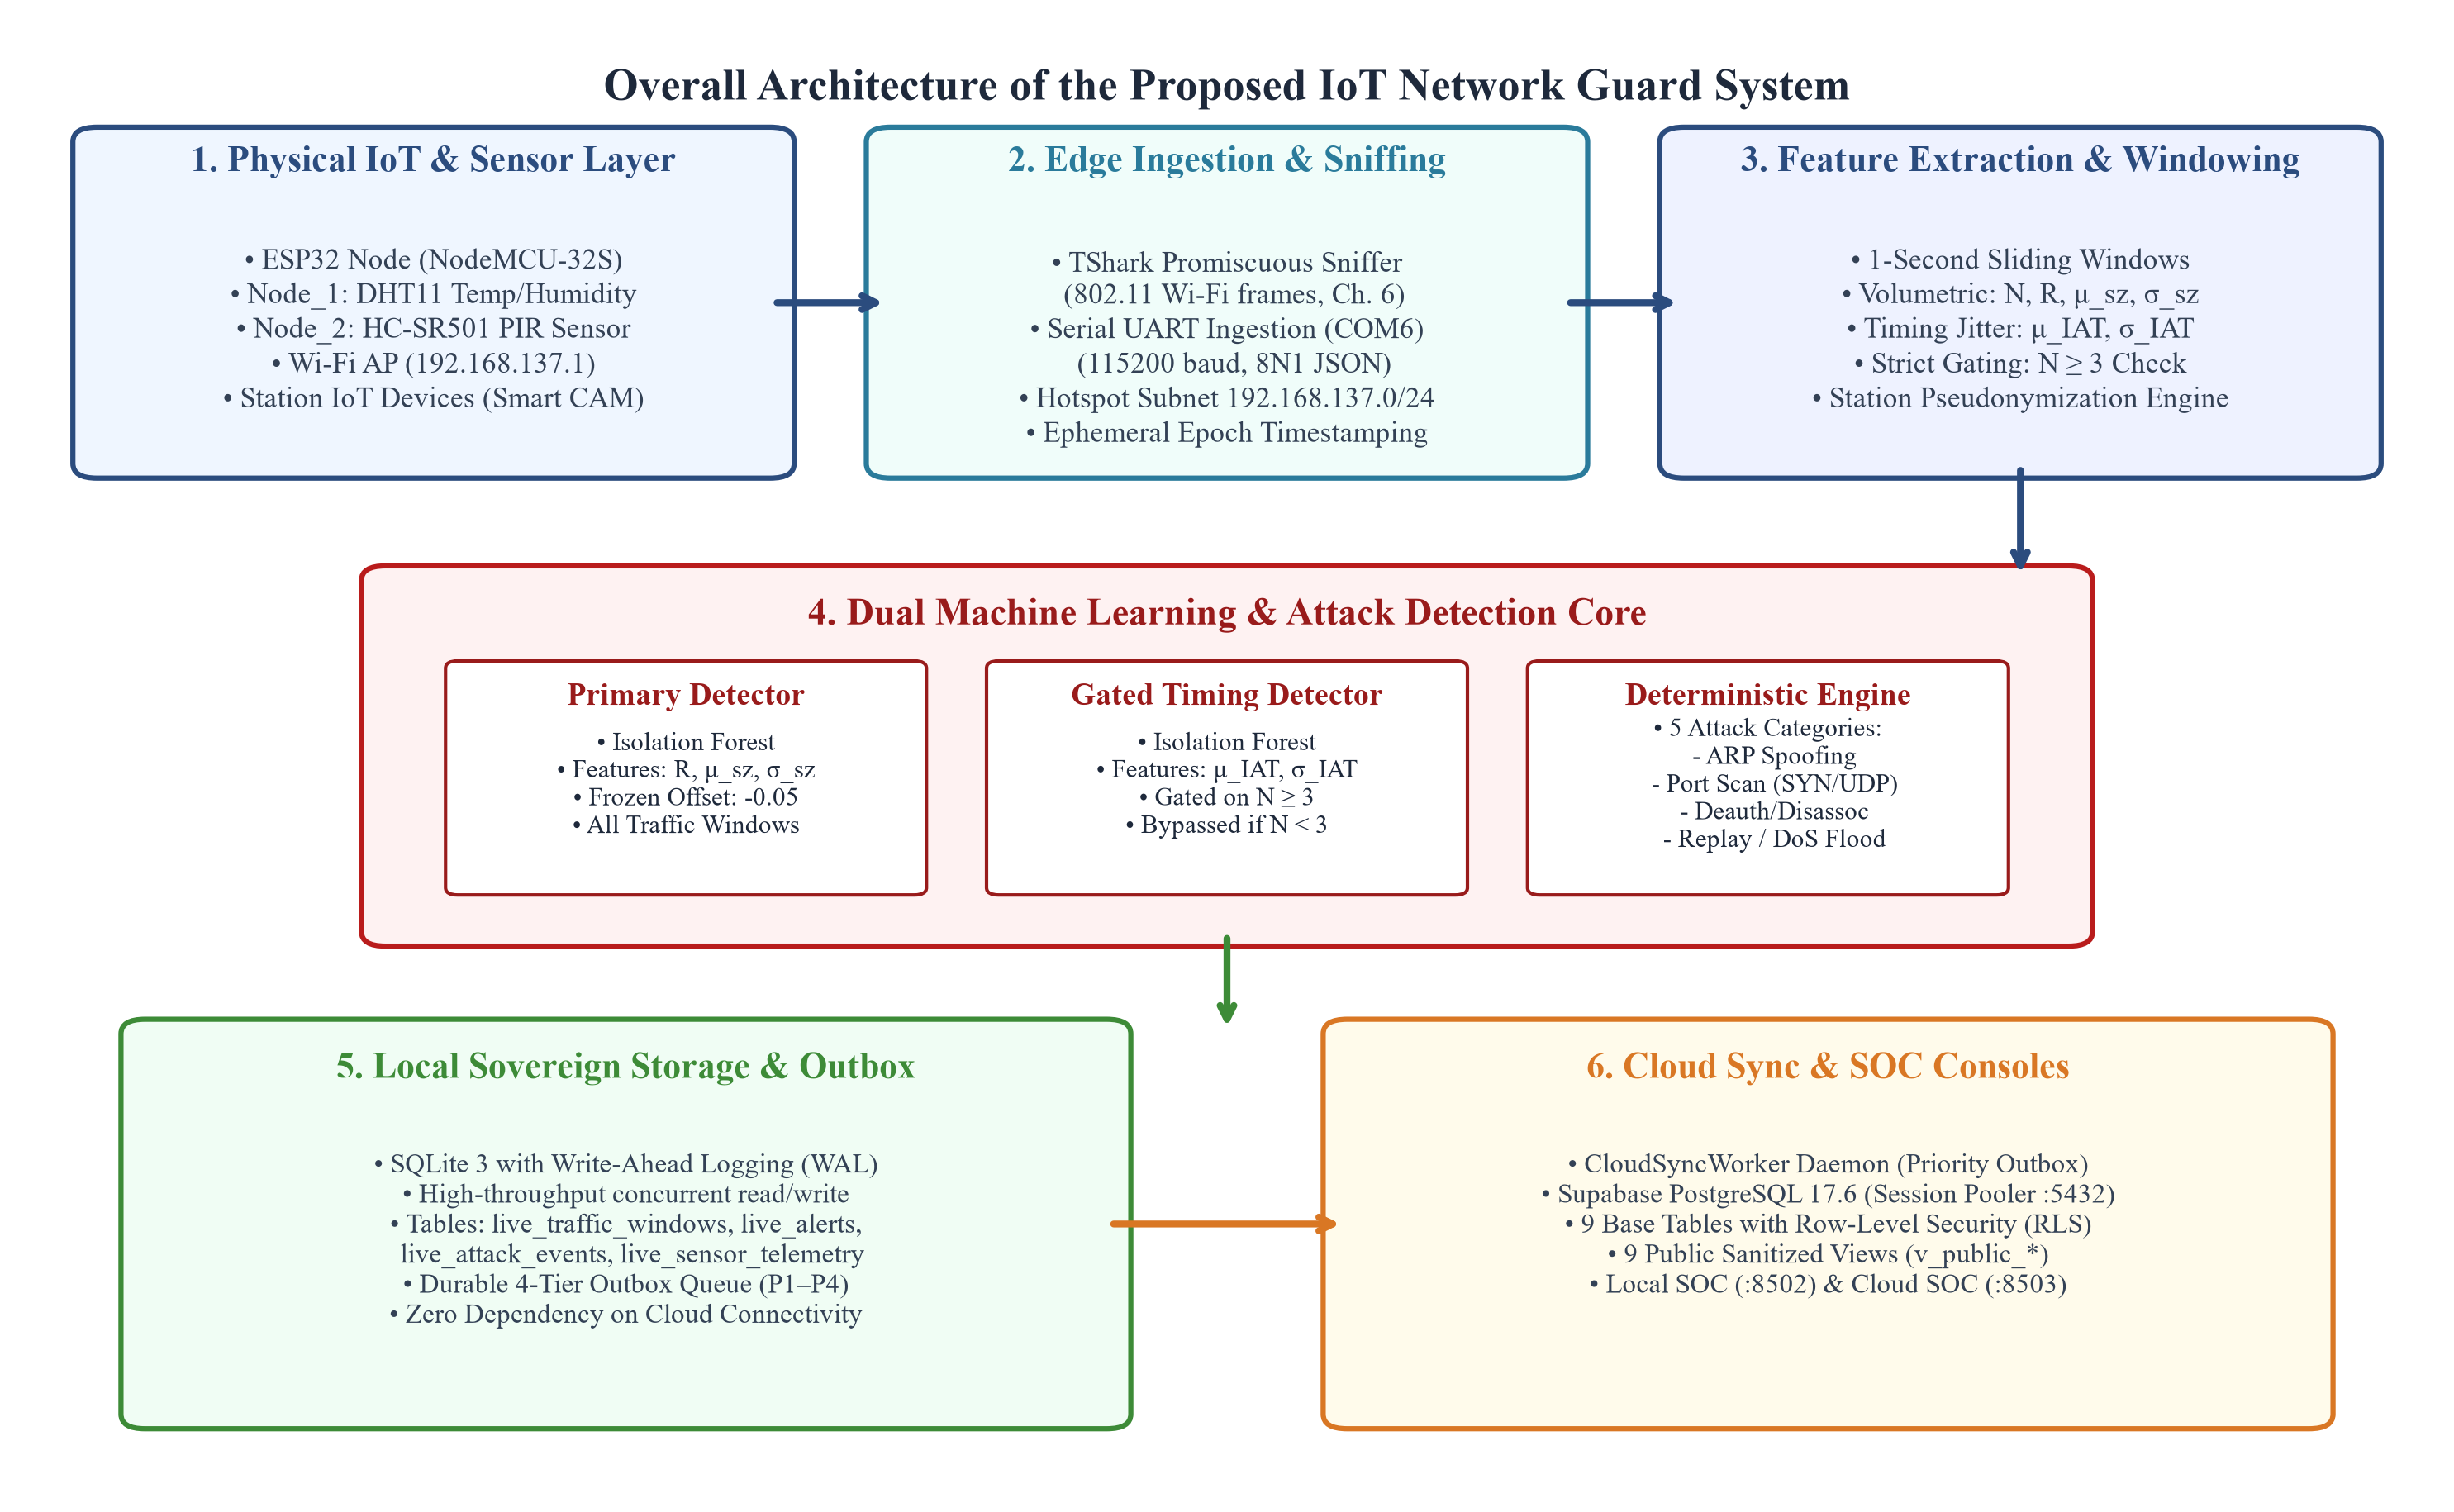
\includegraphics[width=0.92\textwidth]{figures/Figure_3_1_Overall_Architecture.png}
\caption{Overall Architecture of the Proposed IoT Network Guard System}\label{fig:overall_arch}
\end{figure}

As depicted in Figure~\ref{fig:overall_arch}, the system operates across six coordinated architectural tiers:
\begin{enumerate}[leftmargin=*]
    \item \textbf{Physical IoT \& Sensor Layer:} Comprises physical wireless station nodes (commercial smart cameras, IoT microcontrollers) communicating over 802.11b/g/n with a Wi-Fi Access Point (hotspot gateway at 192.168.137.1), alongside an ESP32 hardware probe acquiring physical ambient environmental data (DHT11 temperature/humidity) and physical PIR occupancy events.
    \item \textbf{Edge Ingestion \& Sniffing Layer:} Leverages TShark to intercept raw 802.11 and Ethernet frames across the monitored network interface in promiscuous mode without packet dropping, while concurrently reading serial UART JSON streams from the ESP32 node via COM6 at 115200 baud.
    \item \textbf{Feature Extraction \& Windowing Layer:} Employs a high-throughput stream parser that aggregates raw packet timestamps and lengths into non-overlapping 1-second temporal feature windows, computes statistical metrics, hashes MAC addresses into pseudonyms, and evaluates the mathematical degrees-of-freedom gate.
    \item \textbf{Dual Machine Learning \& Attack Detection Core:} Executes the frozen Dual Isolation Forest pipeline to classify windows as normal or anomalous, while concurrently routing packet headers through the deterministic cyberattack engine to identify specific threat categories.
    \item \textbf{Local Sovereign Storage Layer:} Persists all window features, anomaly alerts, classified attacks, and sensor telemetry directly into a high-concurrency SQLite database operating in Write-Ahead Logging (WAL) mode, guaranteeing zero telemetry loss during internet disruptions.
    \item \textbf{Cloud Synchronization \& SOC Consoles:} A background daemon (\texttt{CloudSyncWorker}) dequeues records from a durable 4-tier priority outbox, delivering encrypted updates via TLS 1.3 to Supabase PostgreSQL 17.6 in Mumbai (ap-south-1). The database exposes nine sanitized, privacy-preserving public views that feed both local (:8502) and cloud-hosted (:8503) Streamlit SOC dashboards.
\end{enumerate}

Figure~\ref{fig:esp32_arch} details the hardware pin connections, sensor interfaces, and internal FreeRTOS firmware architecture of the ESP32 sensing and sniffer node.

\begin{figure}[htbp]
\centering
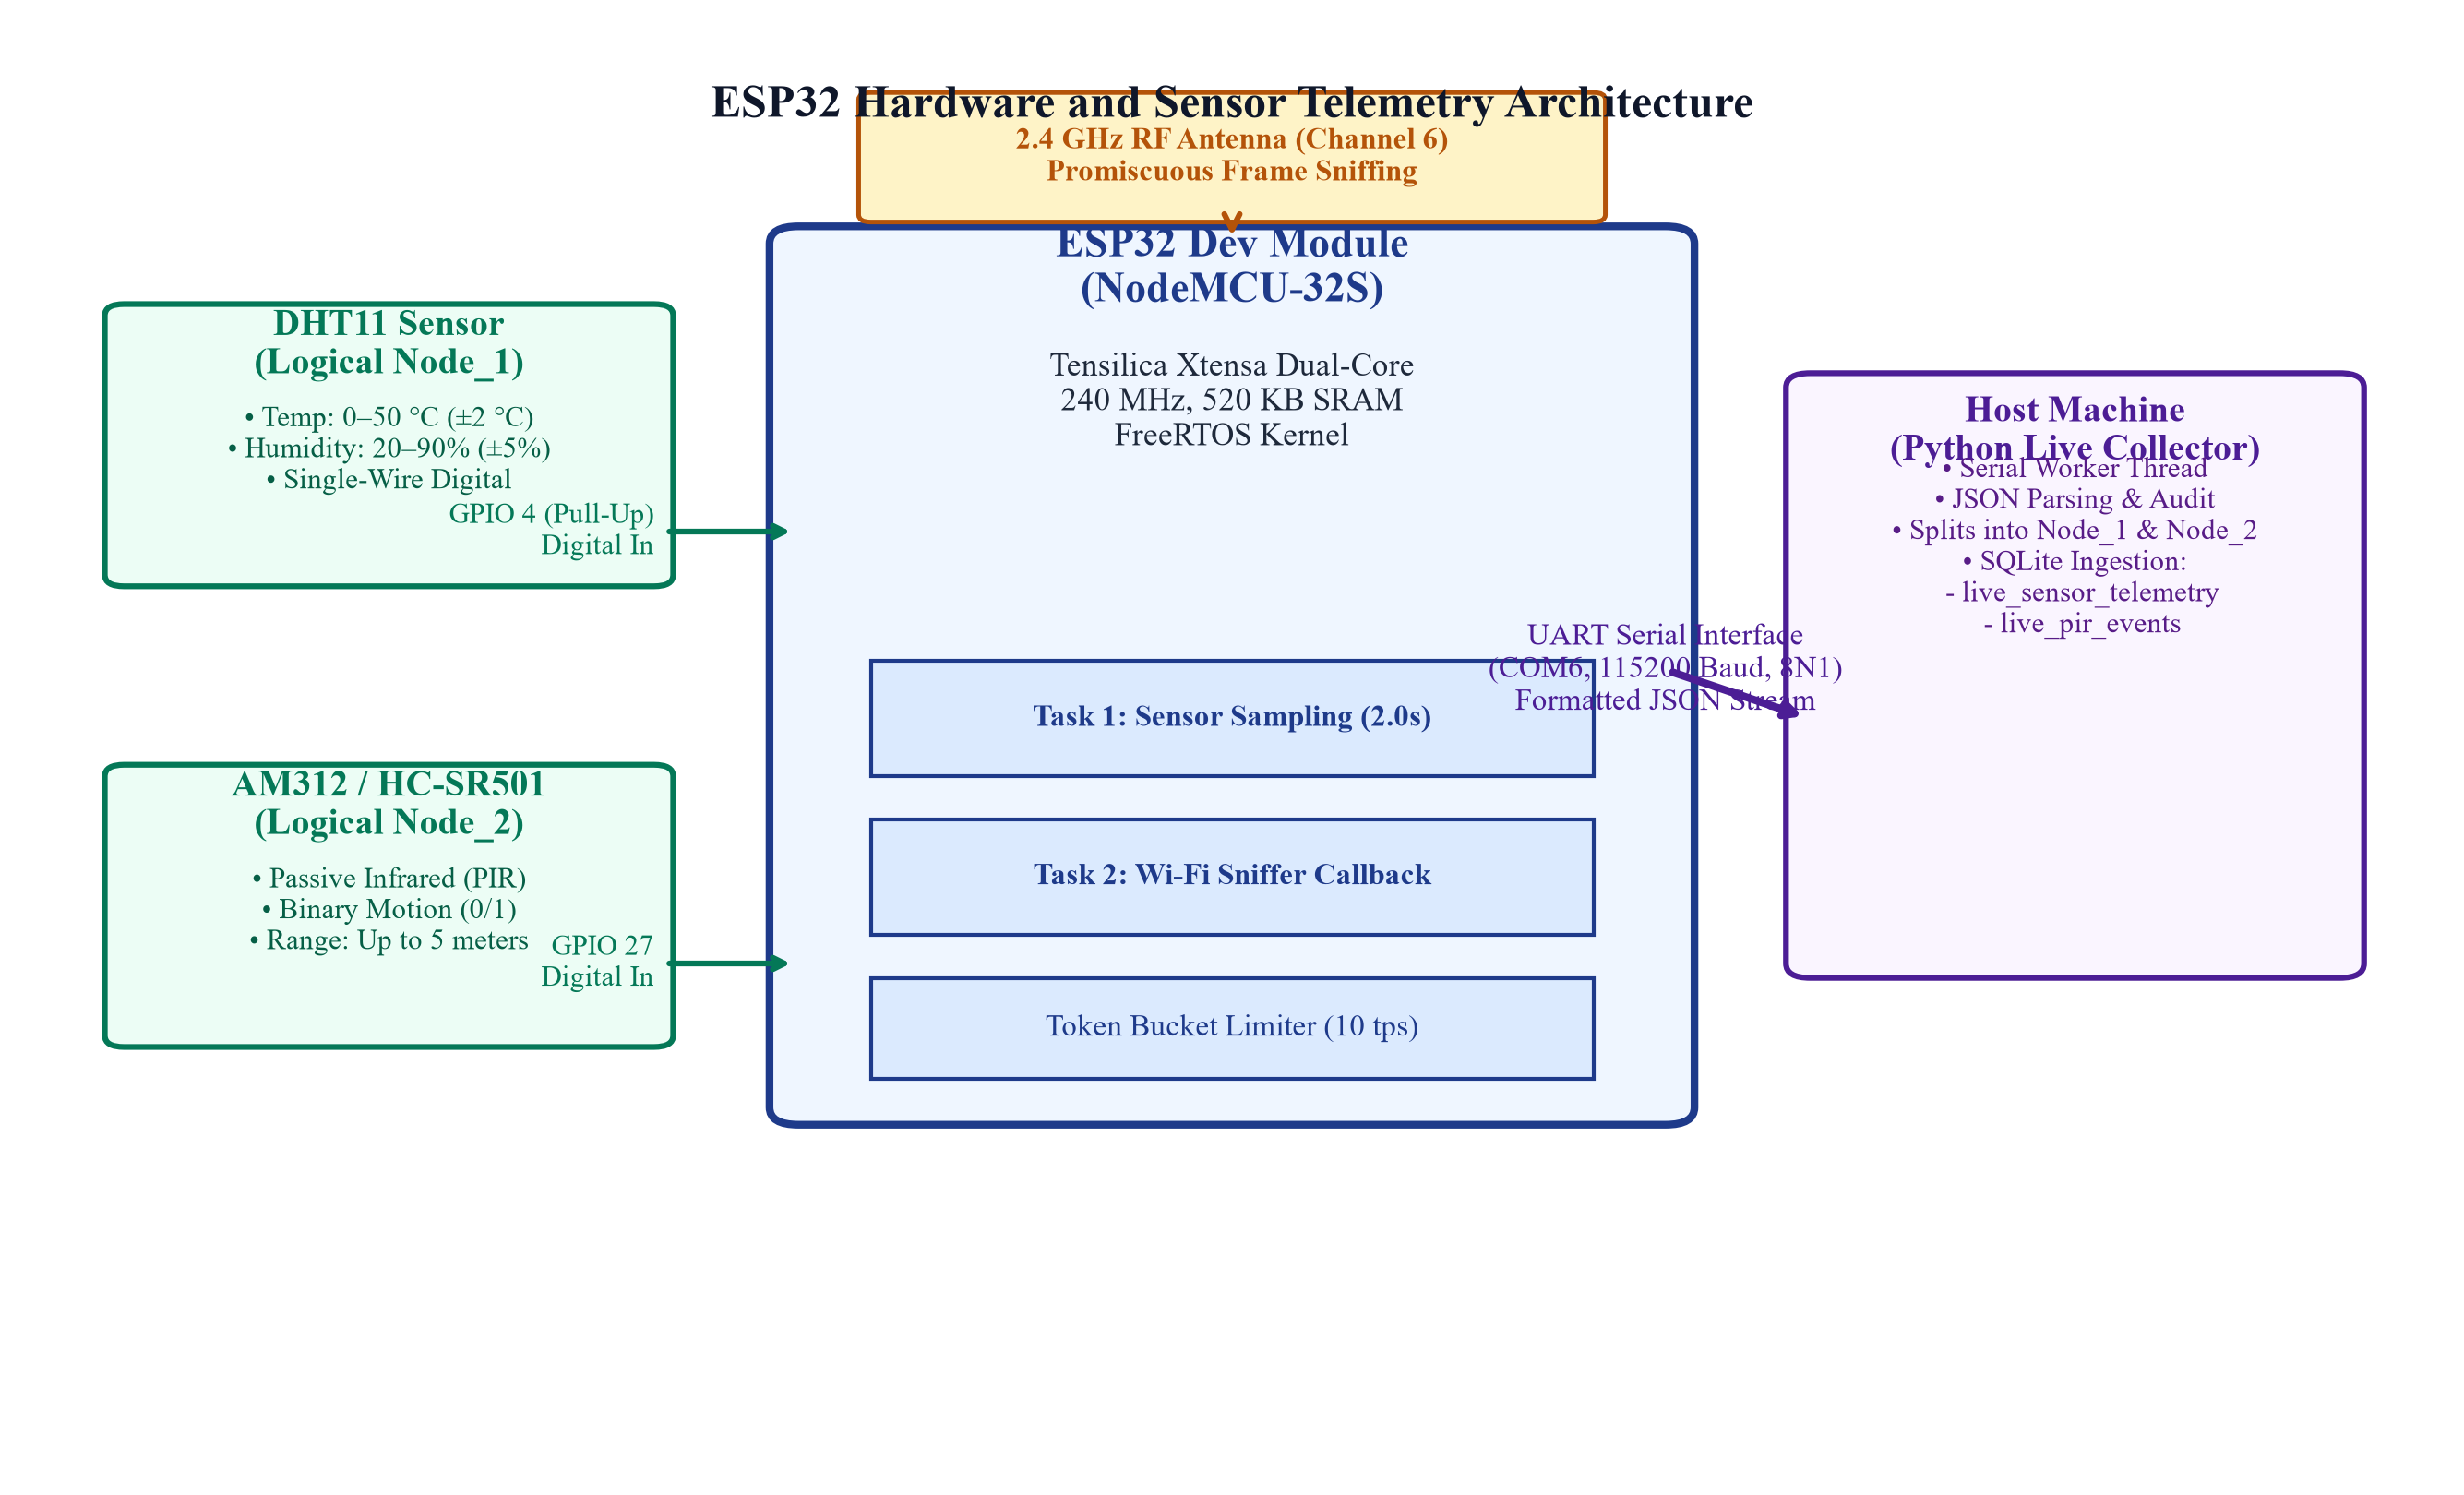
\includegraphics[width=0.88\textwidth]{figures/Figure_3_2_ESP32_Hardware_Architecture.png}
\caption{ESP32 Hardware and Sensor Telemetry Architecture}\label{fig:esp32_arch}
\end{figure}

As illustrated in Figure~\ref{fig:esp32_arch}, the ESP32 node integrates two distinct logical sensing nodes onto a single physical microcontroller:
\begin{itemize}[leftmargin=*]
    \item \textbf{Logical Node\_1 (Environmental Telemetry):} Interfaced to a DHT11 digital temperature and relative humidity sensor connected to GPIO 4 with a 4.7~k$\Omega$ pull-up resistor. The sensor measures temperatures from 0~\textdegree C to 50~\textdegree C ($\pm$2~\textdegree C accuracy) and relative humidity from 20\% to 90\% RH ($\pm$5\% accuracy), sampled periodically every 2000~ms.
    \item \textbf{Logical Node\_2 (Physical Motion Events):} Interfaced to an AM312 / HC-SR501 passive infrared (PIR) motion sensor connected to GPIO 27. The sensor detects human infrared radiating shifts within a 5-meter range, producing binary motion states (0 = quiescent, 1 = motion detected).
    \item \textbf{Promiscuous Management Sniffer Core:} The firmware activates the ESP32 Wi-Fi core in promiscuous sniffer mode locked to 2.4~GHz Channel 6. An internal FreeRTOS queue (depth 32) buffers 802.11 management frames (Subtype 10: Disassociation, Subtype 12: Deauthentication). To prevent serial bus saturation during flooding attacks, a token bucket rate limiter strictly caps serial frame reporting to 10 events per second.
    \item \textbf{Serial Telemetry Interface:} The ESP32 formats validated readings into structured JSON objects transmitted across the CP2102 USB-to-UART bridge to the host machine at 115200 baud, 8 data bits, no parity, and 1 stop bit (8N1).
\end{itemize}

\subsection{Hardware and Software Requirements}
Table~\ref{tab:hardware_specs} summarizes the complete hardware components, interface pins, and operating specifications.

\begin{table}[htbp]
\centering
\caption{Hardware Components and Environmental Sensing Specifications}\label{tab:hardware_specs}
\vspace{6pt}
\begin{tabularx}{\textwidth}{|p{2.2cm}|p{2.4cm}|p{2.0cm}|p{1.6cm}|p{2.0cm}|X|}
\hline
\rowcolor{black!10}
\textbf{Component} & \textbf{Model / Spec} & \textbf{Interface / Pin} & \textbf{Voltage} & \textbf{Rate / Baud} & \textbf{Functional Purpose} \\
\hline
MCU & ESP32 Dev Module (NodeMCU-32S) & USB / UART / 2.4 GHz RF & 3.3 V / 5 V USB & 240 MHz dual-core & Sensor acquisition \& 802.11 sniffer core \\
\hline
Environmental Sensor & DHT11 Digital Sensor & GPIO 4 (Digital In + Pull-up) & 3.3 V DC & 0.5 Hz (2000 ms) & Captures ambient temp (0--50\textdegree C) \& humidity (20--90\%) \\
\hline
Motion Sensor & AM312 / HC-SR501 PIR & GPIO 27 (Digital In) & 3.3 V DC & Event interrupt & Detects physical room occupancy / intrusion \\
\hline
Wi-Fi Sniffer Radio & Tensilica Xtensa Wi-Fi Core & PCB Trace Antenna & 3.3 V DC & Promiscuous Ch. 6 (2.4 GHz) & Sniffs 802.11 deauth/disassoc management frames \\
\hline
Host Workstation & x86-64 Host (Win 11, 16 GB RAM) & COM6 Serial / Wi-Fi Adapter & 110--240 V AC & 115200 baud / 1 Gbps & Executes live collector, ML pipeline, \& local SOC \\
\hline
\end{tabularx}
\end{table}

The software infrastructure is developed entirely in Python 3.12, utilizing established scientific computing, machine learning, and database libraries. Table~\ref{tab:software_stack} details the complete software stack, dependency libraries, versions, and operational roles.

\begin{table}[htbp]
\centering
\caption{Software Stack, Frameworks, and Deployment Dependencies}\label{tab:software_stack}
\vspace{6pt}
\begin{tabularx}{\textwidth}{|p{2.2cm}|p{2.2cm}|p{1.6cm}|p{2.2cm}|X|}
\hline
\rowcolor{black!10}
\textbf{Layer} & \textbf{Framework} & \textbf{Version} & \textbf{Context} & \textbf{Key Functional Responsibility} \\
\hline
Runtime & Python & 3.12.x & Workstation Host & Core execution runtime for collector, ML, and dashboard \\
\hline
Machine Learning & scikit-learn & 1.5.x & Inference Pipeline & Implements Dual Isolation Forest ensembles and imputers \\
\hline
Data Processing & pandas \& numpy & 2.2.x / 1.26.x & Feature Extractor & Vectorized 1-second feature windowing and array math \\
\hline
Packet Sniffing & TShark (Wireshark) & 4.2.x & Network Thread & Promiscuous frame dissection and epoch timestamp extraction \\
\hline
Local Database & SQLite 3 & 3.45.x (WAL) & Edge Persistence & High-concurrency sovereign local storage for all telemetry \\
\hline
Cloud Database & Supabase Postgres & 17.6 (Mumbai) & Cloud Backend & Cloud database host with RLS, connection pooler, \& views \\
\hline
Database Driver & psycopg2-binary & 2.9.x & Sync Worker & Direct PostgreSQL driver connecting to Supabase pooler (:5432) \\
\hline
SOC Visualization & Streamlit & 1.38.x & SOC Consoles & Interactive Security Operations Center dashboard UI \\
\hline
\end{tabularx}
\end{table}

\section{IMPLEMENTATION}
The operational workflow of IoT Network Guard is executed through two concurrent threads in the background daemon (\texttt{src/live\_collector.py}): the Network Thread responsible for live packet interception and dual ML inference, and the Serial Thread responsible for ESP32 hardware telemetry ingestion.

\subsection{Algorithm}
Figure~\ref{fig:packet_capture} illustrates the five-stage packet capture, temporal slicing, and feature extraction workflow executed by the Network Thread.

\begin{figure}[htbp]
\centering
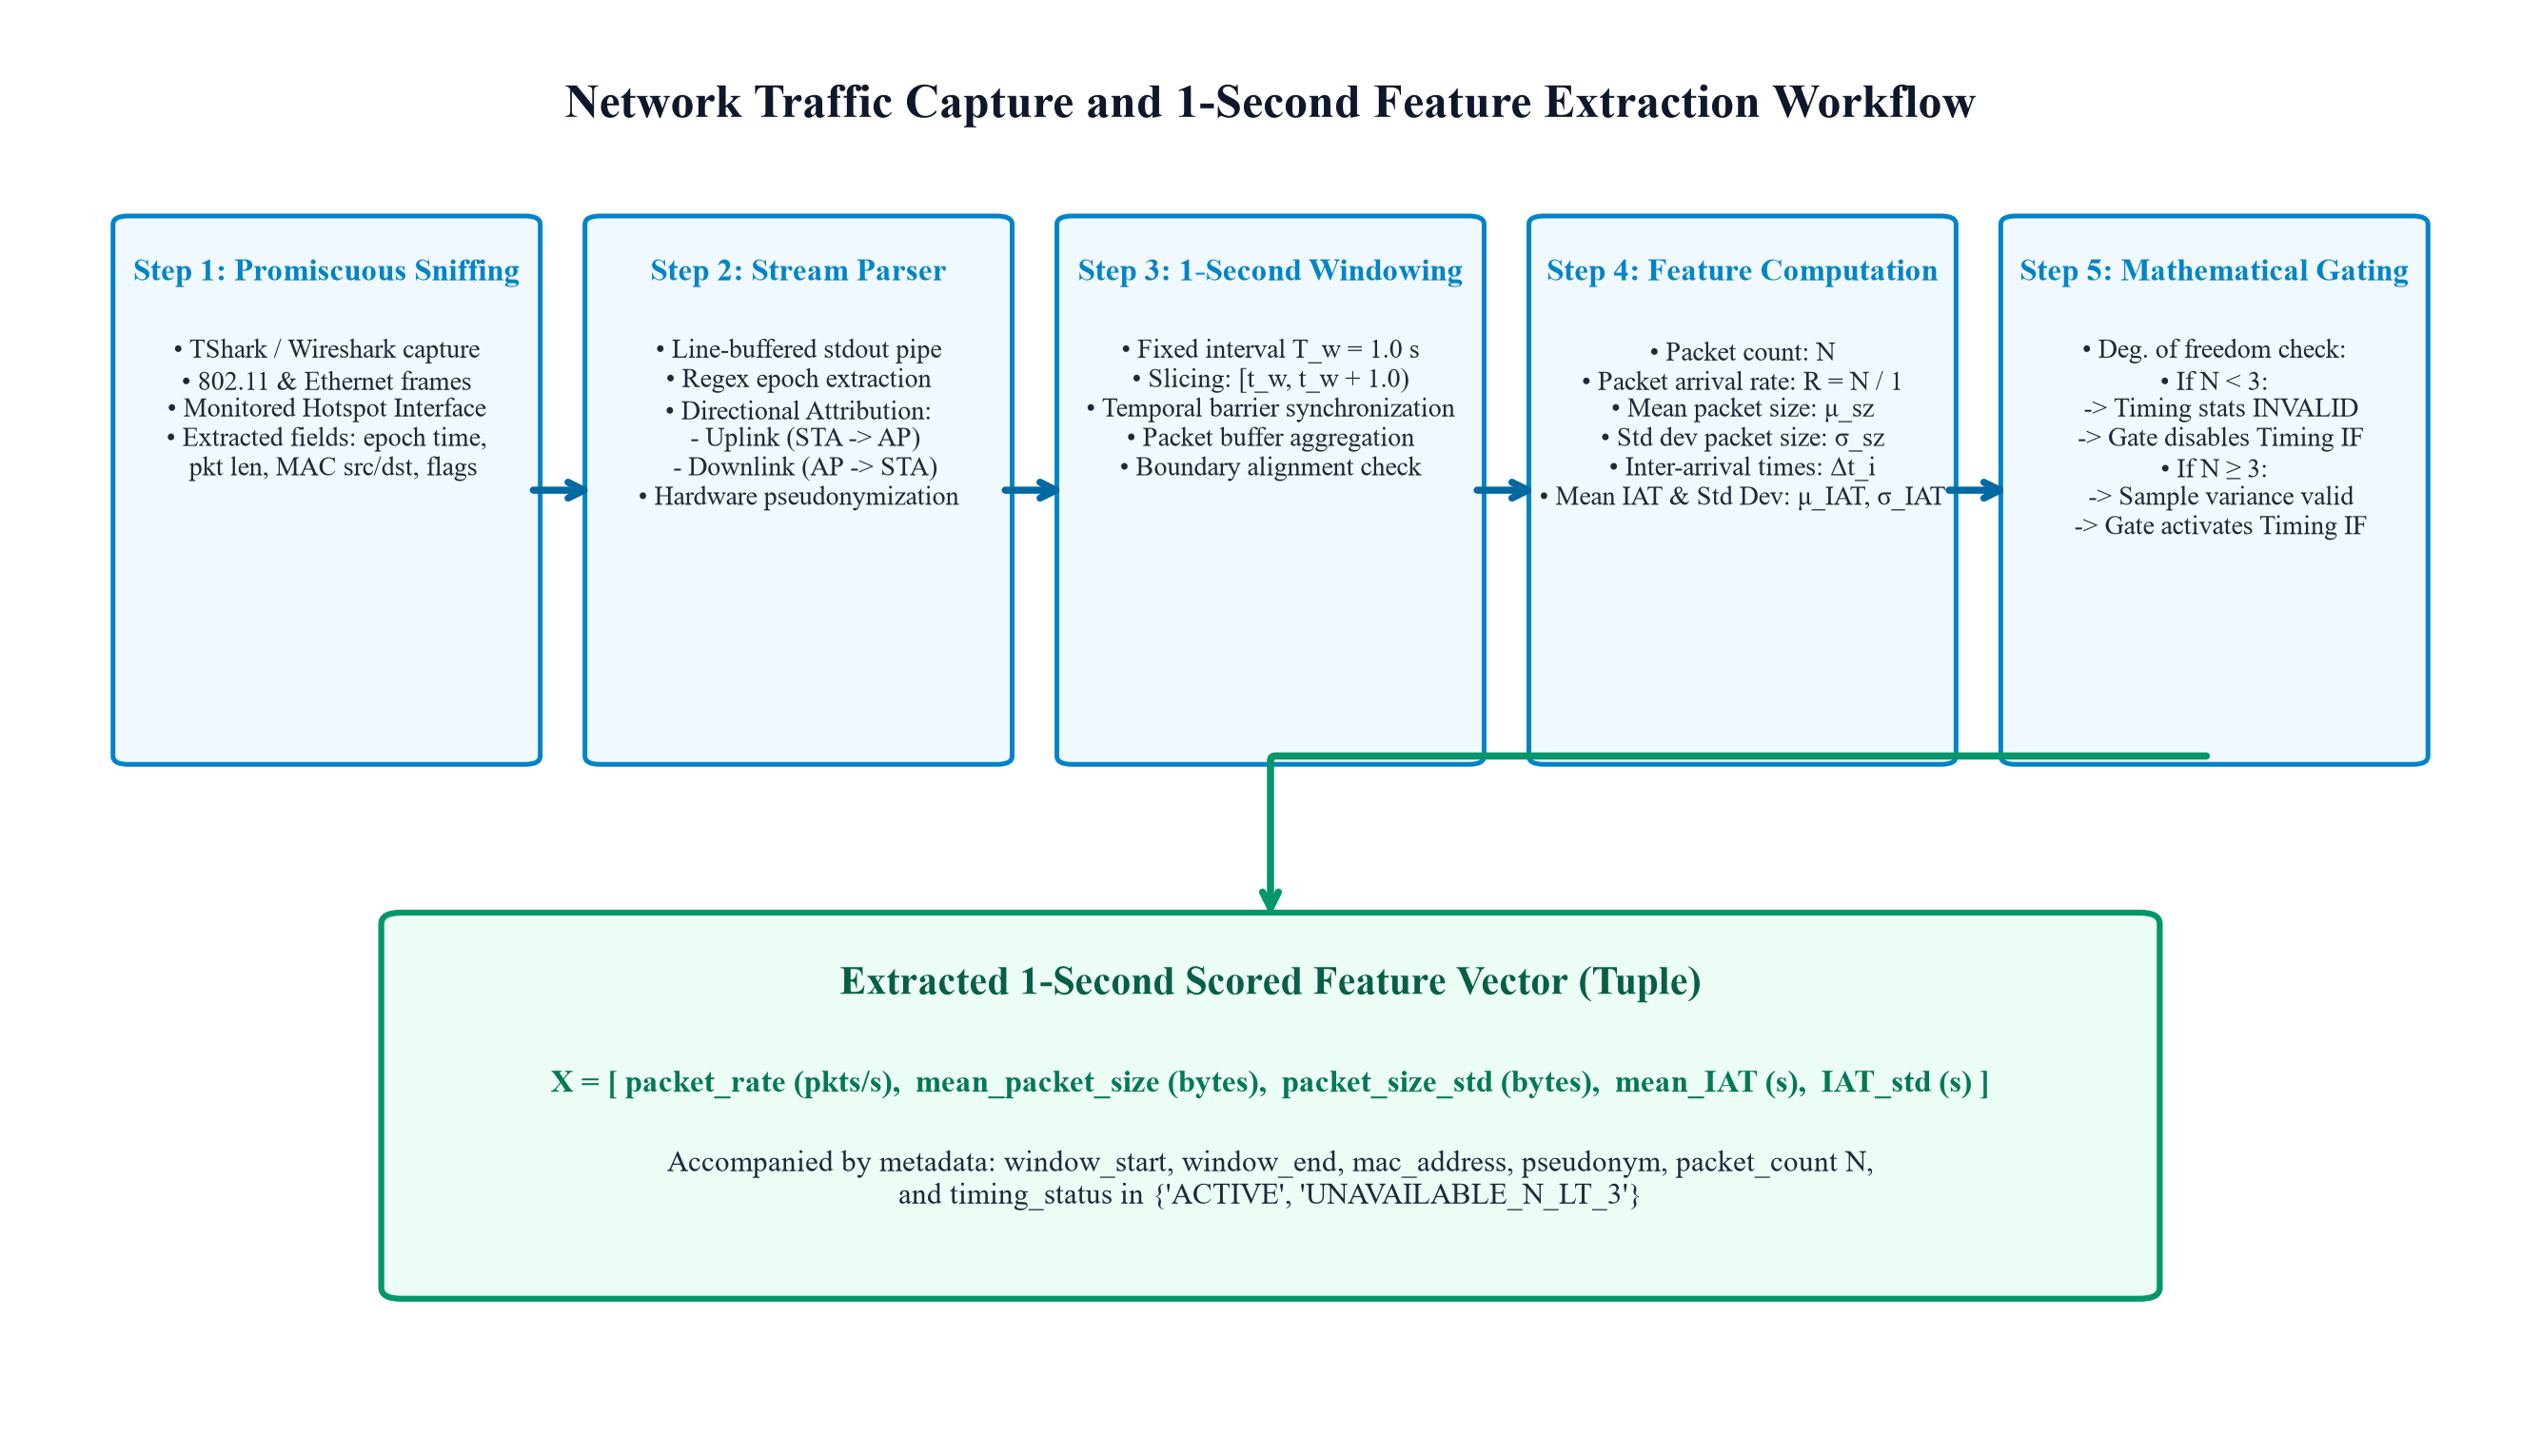
\includegraphics[width=0.90\textwidth]{figures/Figure_3_3_Packet_Capture_Workflow.png}
\caption{Network Traffic Capture and 1-Second Feature Extraction Workflow}\label{fig:packet_capture}
\end{figure}

The workflow proceeds in five sequential stages:
\begin{enumerate}[leftmargin=*]
    \item \textbf{Promiscuous Sniffing:} TShark is launched as a subprocess bound to the monitored wireless interface with an unbuffered stdout pipe. For every observed frame, TShark extracts the frame arrival epoch, packet length, source MAC, destination MAC, IP addresses, transport ports, and protocol flags.
    \item \textbf{Stream Parsing \& Attribution:} The extractor parses the stdout pipe line-by-line using compiled regular expressions. Packets are directionally classified as Uplink (station transmitting to AP) or Downlink (AP transmitting to station). Hardware MAC addresses are mapped to privacy-preserving station pseudonyms (e.g., Station\_A, Station\_B, Station\_C) using deterministic cryptographic hashing.
    \item \textbf{1-Second Temporal Window Slicing:} Packets are buffered into fixed 1.0-second sliding windows bounded by $[t_k, t_k + 1.0)$. When the stream timestamp crosses the window boundary, the buffer is locked and dispatched for feature calculation.
    \item \textbf{Feature Vector Computation:} The extractor computes the six core features: packet count $N$, arrival rate $R$, mean packet size $\mu_{\text{size}}$, size standard deviation $\sigma_{\text{size}}$, mean inter-arrival time $\mu_{\text{IAT}}$, and IAT standard deviation $\sigma_{\text{IAT}}$.
    \item \textbf{Mathematical Gating:} The sample size $N$ is audited. If $N < 3$, the window is tagged with \texttt{timing\_status = 'UNAVAILABLE\_N\_LT\_3'}, preventing the calculation of invalid sample variance and instructing the ML pipeline to bypass timing evaluation. If $N \ge 3$, \texttt{timing\_status = 'ACTIVE'}.
\end{enumerate}

Figure~\ref{fig:dual_ml_arch} diagrams the Dual Isolation Forest inference architecture, demonstrating how sample gating decouples volumetric evaluation from timing jitter analysis.

\begin{figure}[htbp]
\centering
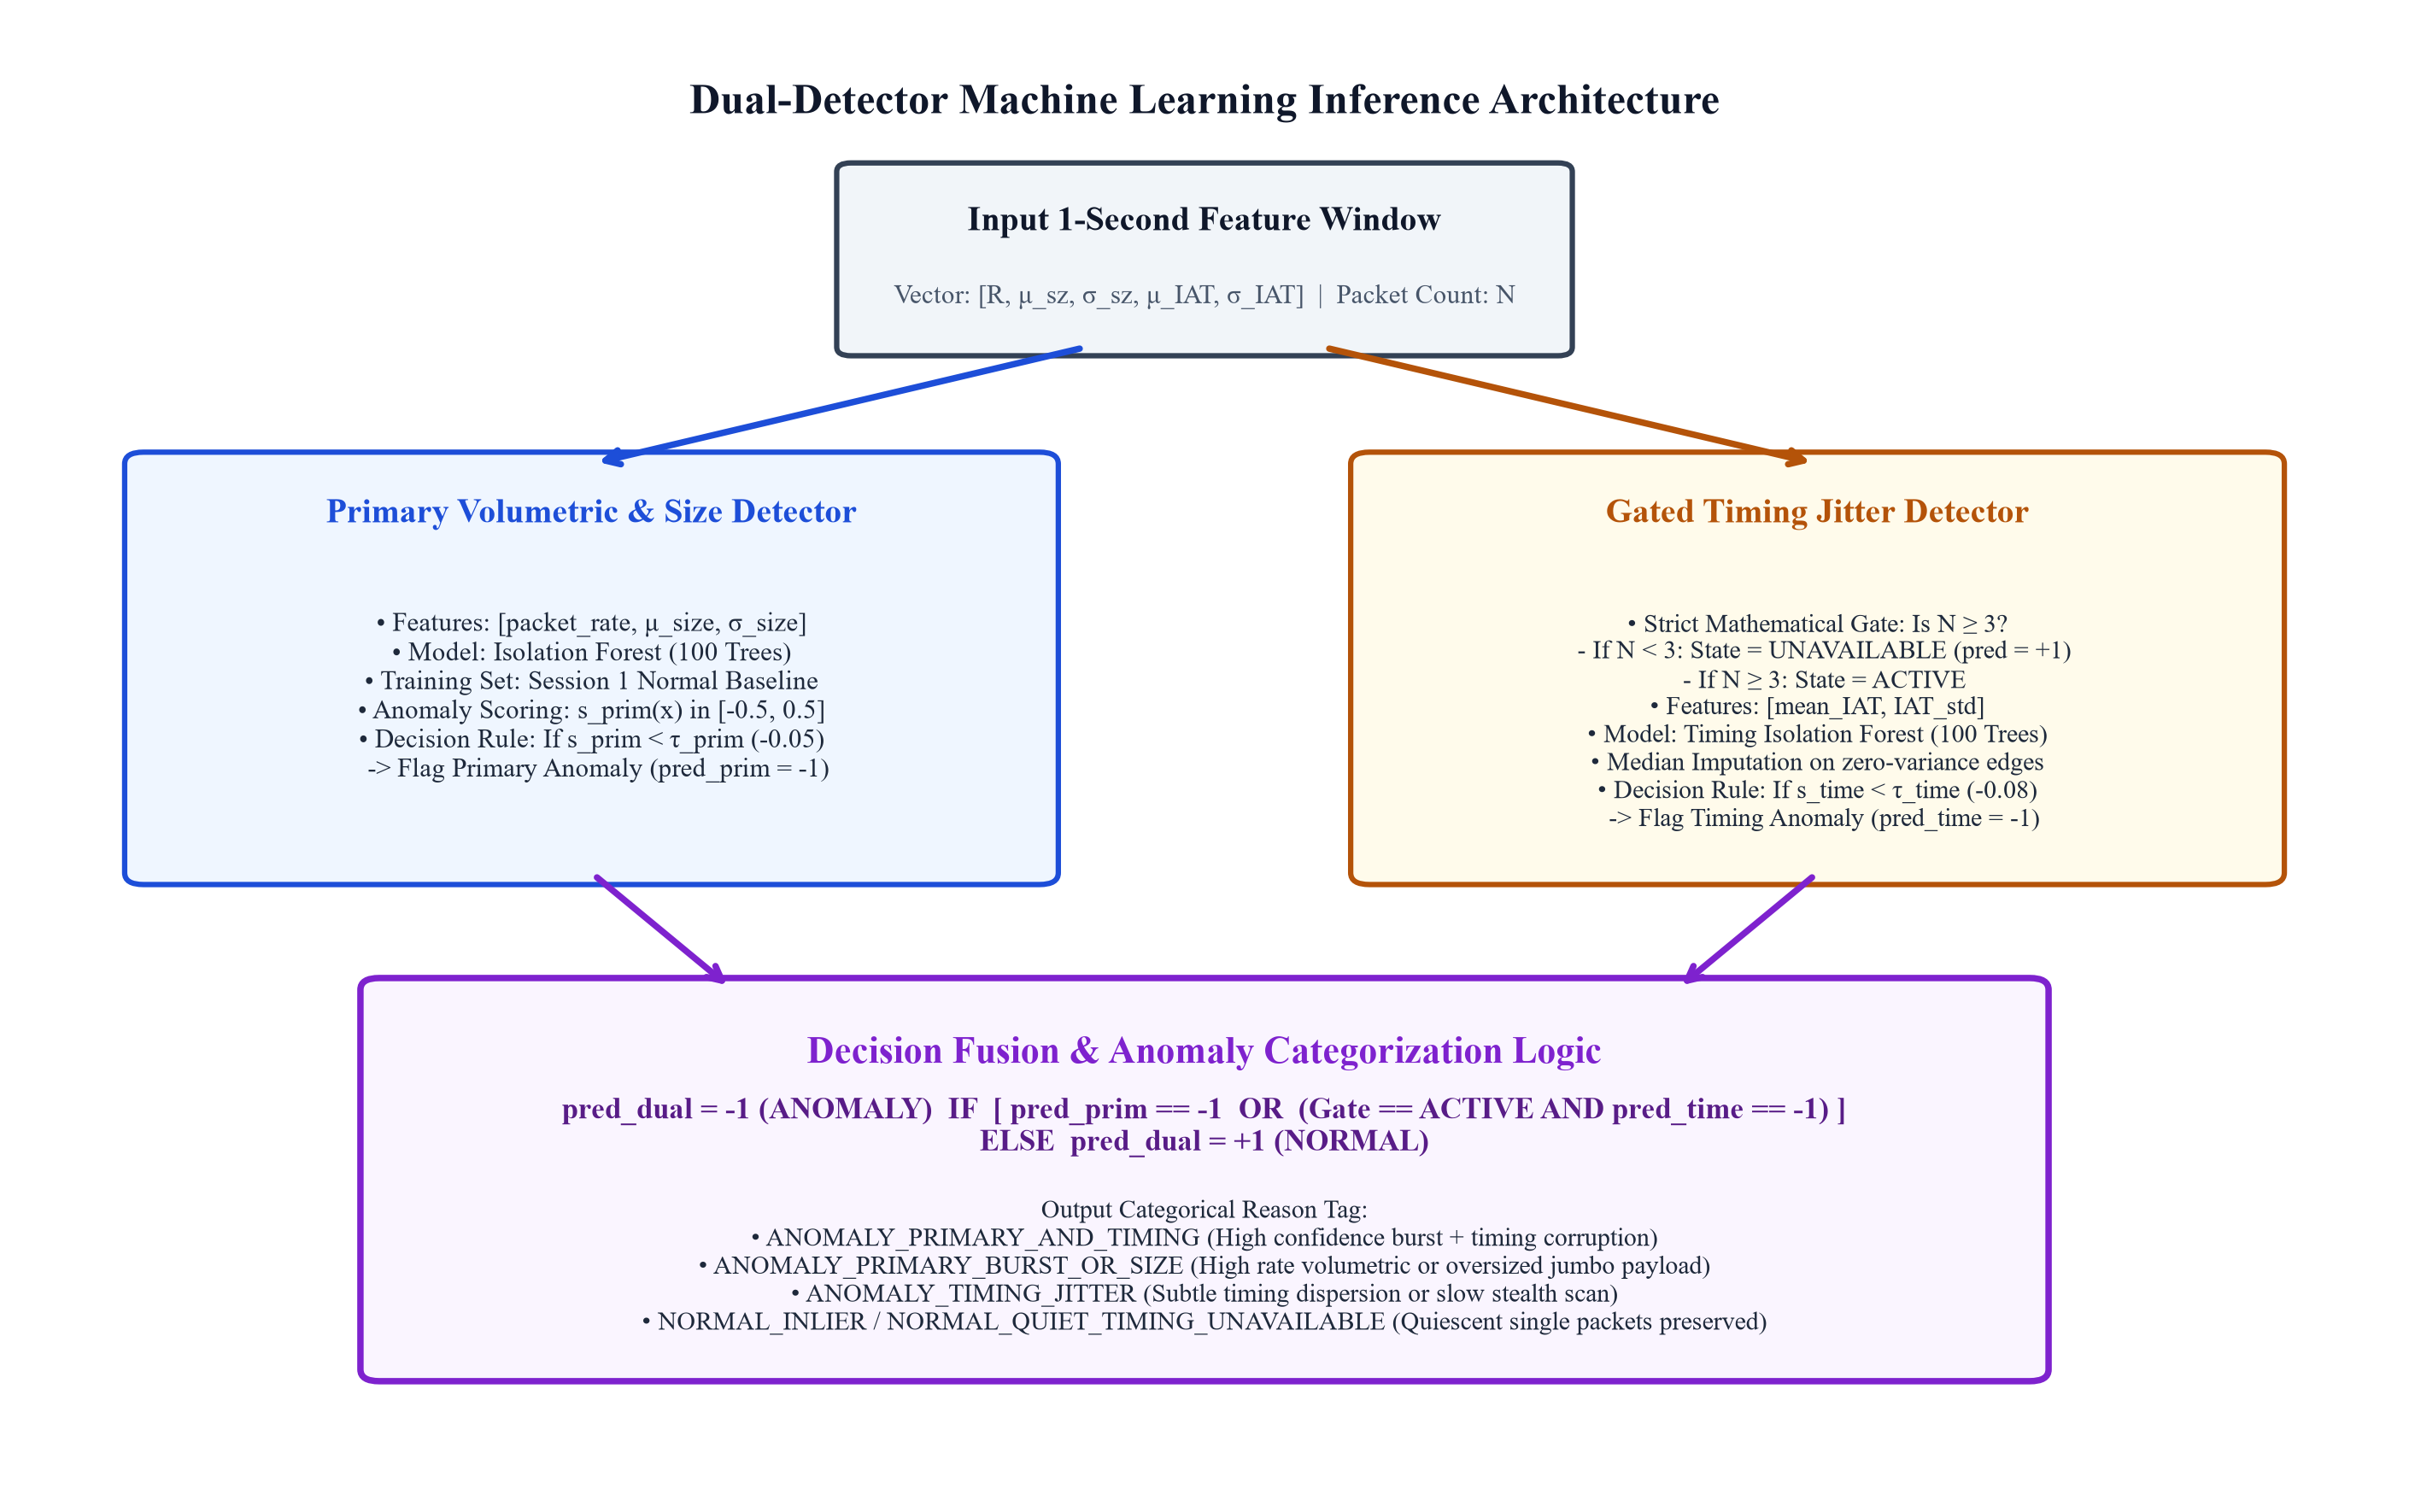
\includegraphics[width=0.92\textwidth]{figures/Figure_3_4_Dual_Detector_ML_Architecture.png}
\caption{Dual-Detector Machine Learning Inference Architecture}\label{fig:dual_ml_arch}
\end{figure}

The machine learning pipeline is governed by Algorithm~3.1. Both detectors are trained strictly on legitimate Session 1 baseline traffic using 100 trees, a contamination factor of 0.05, and \texttt{random\_state = 42}. Crucially, the models are frozen and re-created deterministically from training data on collector initialization, guaranteeing zero runtime drift or unintended threshold corruption.

\begin{lstlisting}[language=Python,caption={Algorithm 3.1: Gated Dual-Detector Machine Learning Inference Procedure},label={alg:dual_detector}]
# Algorithm 3.1: Gated Dual-Detector Machine Learning Inference Procedure
# Input:  Feature Vector X = [R, mu_size, sigma_size, mu_IAT, sigma_IAT], Count N
#         Primary Detector clf_prim, Timing Detector clf_time, Imputer imp_time
#         Decision Thresholds: tau_prim = -0.05, tau_time = -0.08
# Output: Dual Prediction pred_dual in {-1, +1}, Categorical Reason dual_reason

# Step 1: Primary Volumetric / Size Evaluation (Evaluated on ALL windows)
X_prim = [ X.R, X.mu_size, X.sigma_size ]
s_prim = clf_prim.decision_function(X_prim)
pred_prim = -1 if (s_prim < tau_prim) else +1

# Step 2: Mathematical Gating & Timing Evaluation
if N < 3:
    pred_time = +1  # Inlier default (prevents division-by-zero spurious alarms)
    timing_status = 'UNAVAILABLE_N_LT_3'
    s_time = float('nan')
else:
    timing_status = 'ACTIVE'
    X_time = imp_time.transform([ [X.mu_IAT, X.sigma_IAT] ])
    s_time = clf_time.decision_function(X_time)
    pred_time = -1 if (s_time < tau_time) else +1

# Step 3: Combined Decision Fusion & Categorical Reason Tagging
if pred_prim == -1 and pred_time == -1:
    pred_dual, dual_reason = -1, 'ANOMALY_PRIMARY_AND_TIMING'
elif pred_prim == -1:
    pred_dual, dual_reason = -1, 'ANOMALY_PRIMARY_BURST_OR_SIZE'
elif timing_status == 'ACTIVE' and pred_time == -1:
    pred_dual, dual_reason = -1, 'ANOMALY_TIMING_JITTER'
else:
    pred_dual = +1
    dual_reason = 'NORMAL_QUIET_TIMING_UNAVAILABLE' if (N < 3) else 'NORMAL_INLIER'

return pred_dual, dual_reason, s_prim, s_time
\end{lstlisting}

While the Dual Isolation Forest detects statistical deviations without requiring pre-configured attack signatures, operational security personnel require actionable threat classification. The system integrates a deterministic cyberattack engine (\texttt{src/attack\_detector.py}) that evaluates five distinct threat categories:
\begin{enumerate}[leftmargin=*]
    \item \textbf{Denial-of-Service (DoS) / Volumetric Flood:} Evaluates packet arrival rate $R$ and volumetric density. If $R$ exceeds calibrated baseline bounds by $>$300\% (e.g., $R \ge 50$~pkts/s on low-power stations) accompanied by uniform small packet sizes, the engine flags a high-confidence volumetric DoS attack.
    \item \textbf{Reconnaissance / Port Scanning:} Analyzes transport layer destination ports and IP targets across consecutive packets. Vertical scans (probing $\ge$5 distinct ports on a single host within 1 second) and horizontal sweeps (probing the same port across multiple subnet IPs) are identified with confidence ratings up to 0.92.
    \item \textbf{ARP / MAC Spoofing:} Monitors IP-to-MAC resolution tables. If conflicting MAC addresses claim ownership of the default gateway IP (192.168.137.1) or if gratuitous ARP broadcasts exhibit mismatched sender hardware addresses, an impersonation alert is triggered with CRITICAL severity (confidence 0.90).
    \item \textbf{Wi-Fi Deauthentication / Disassociation Flooding:} Evaluates 802.11 management frames reported by the ESP32 sniffer core. If deauthentication (Subtype 12) or disassociation (Subtype 10) frames exceed the threshold of 5 frames/second directed at a single BSSID, a HIGH severity Wi-Fi abuse alert is generated.
    \item \textbf{Replay Attacks:} Detects duplicate packet payloads, stagnant sequence numbers, or regressing timestamps in encrypted sensor sessions, identifying unauthorized packet reinjection with confidence 0.85.
\end{enumerate}

Figure~\ref{fig:storage_cloud} diagrams the local sovereign persistence and cloud synchronization architecture.

\begin{figure}[htbp]
\centering
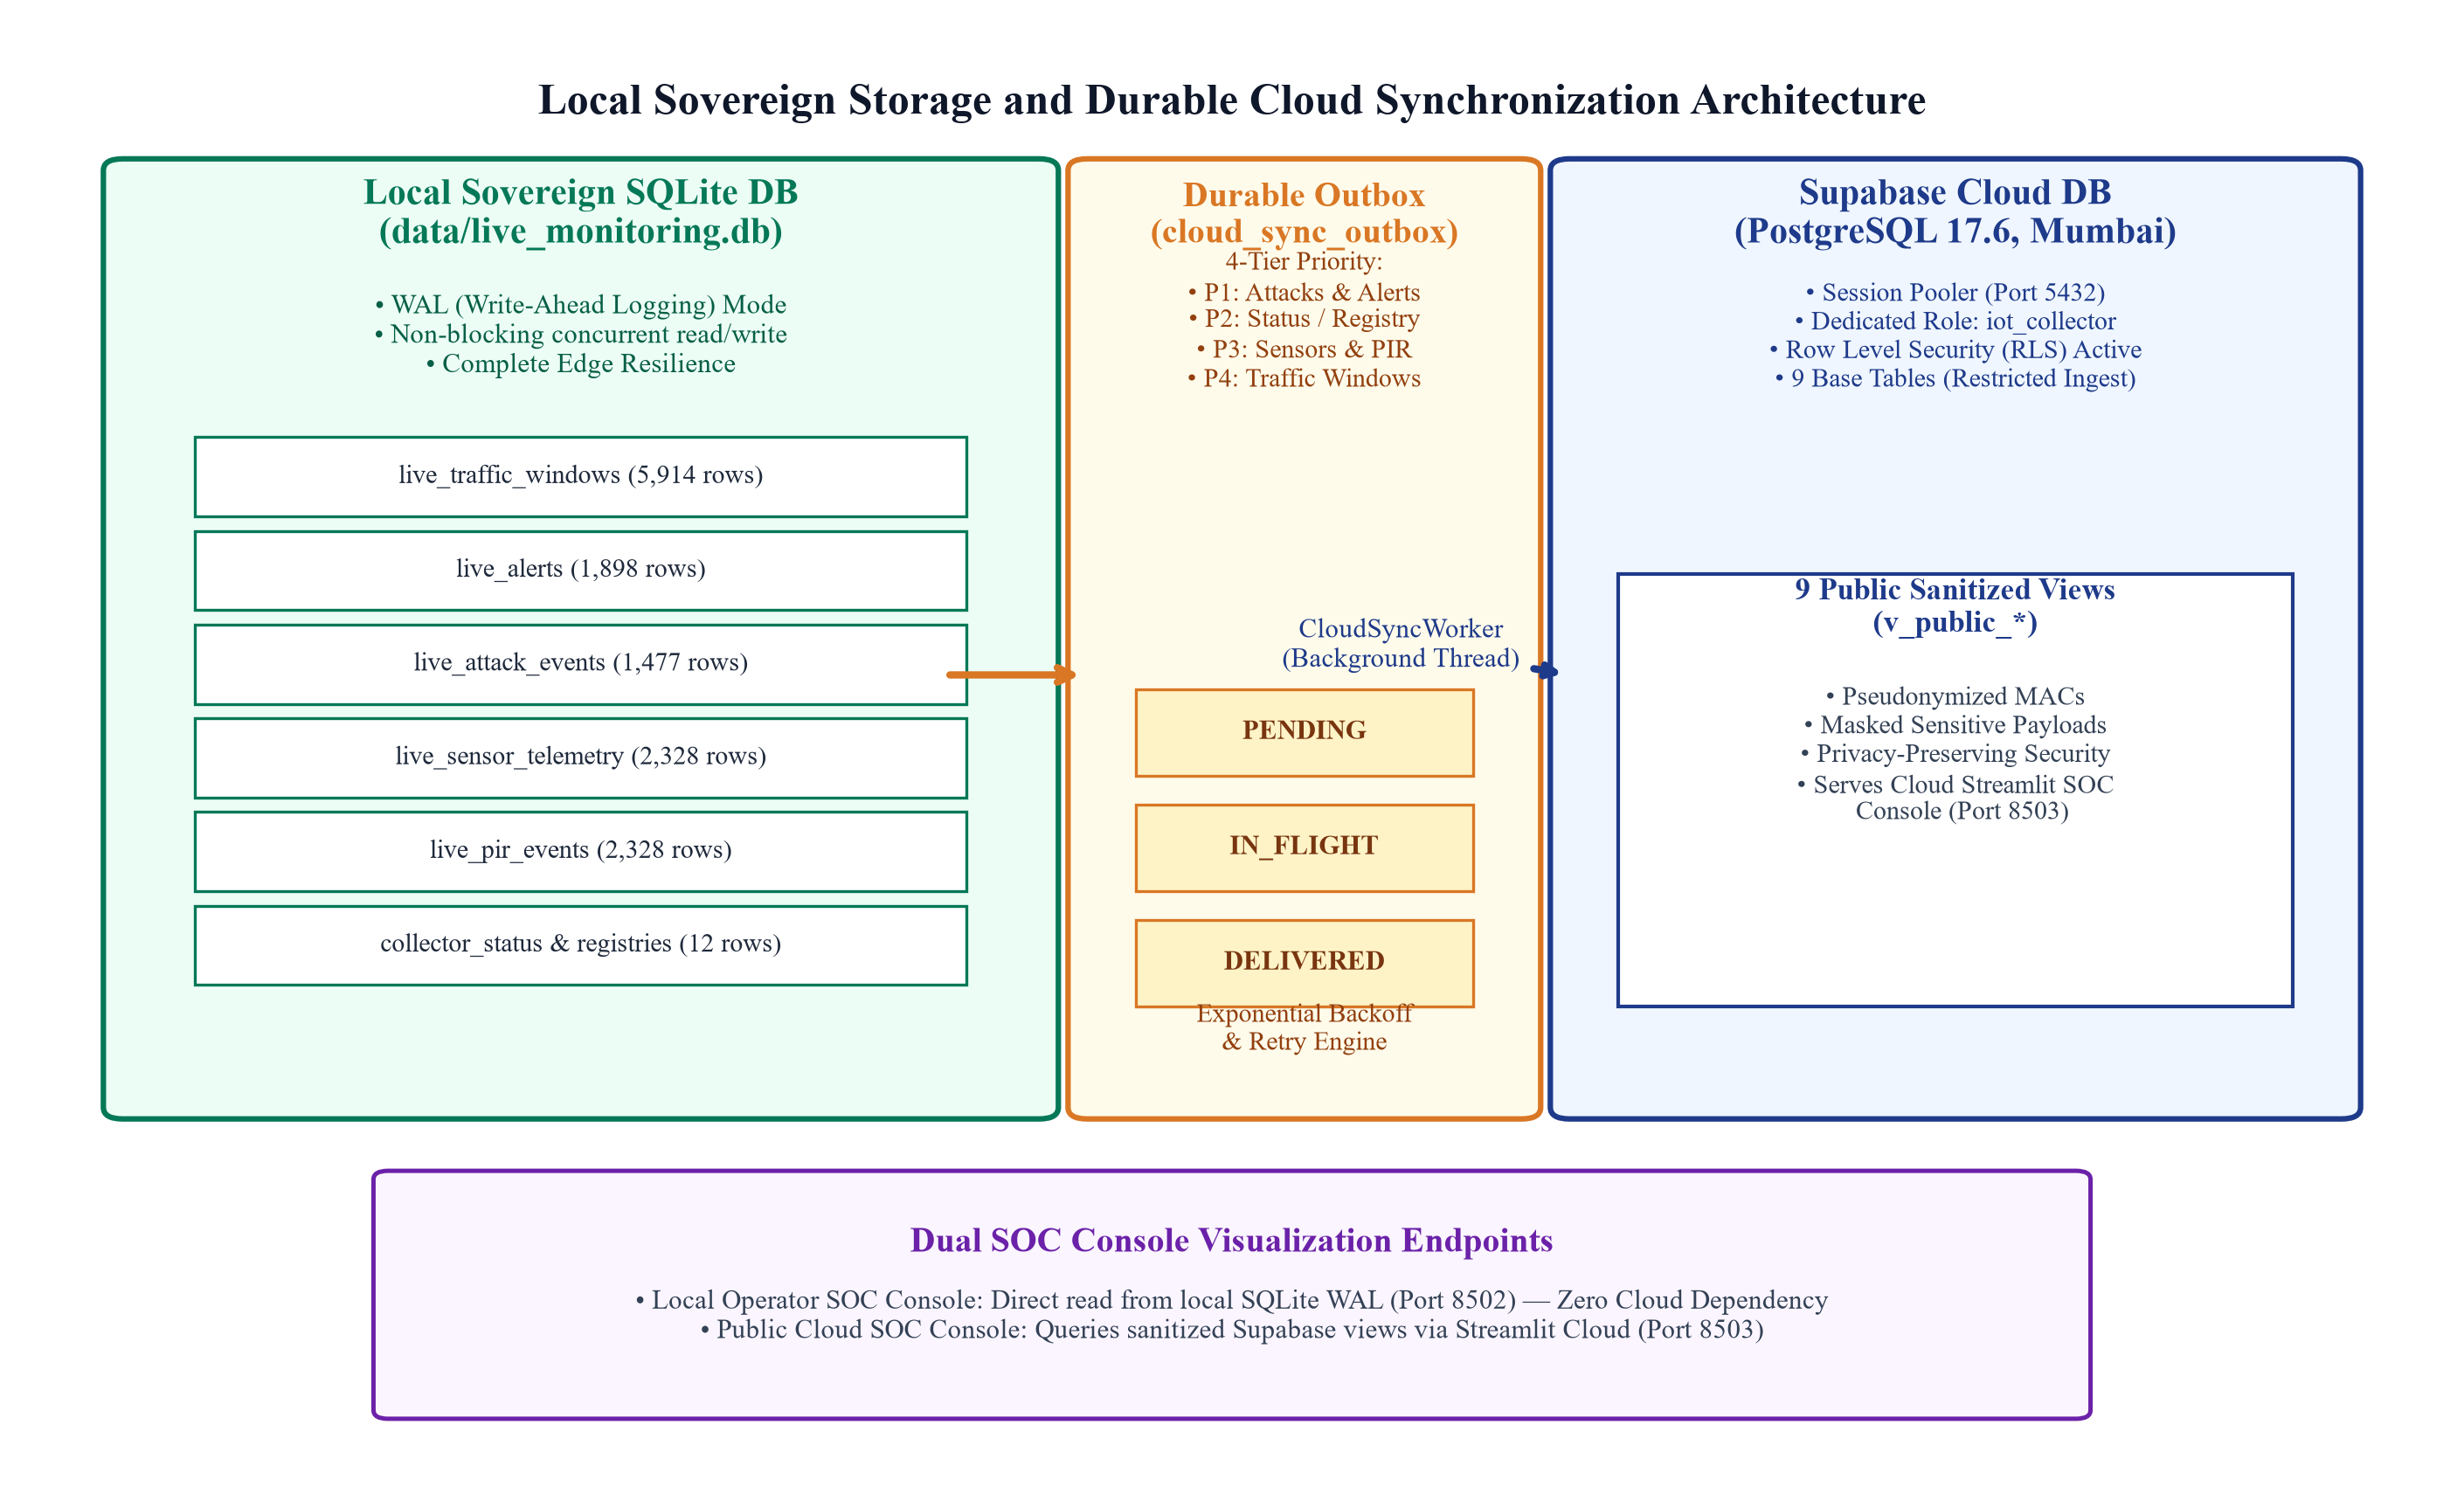
\includegraphics[width=0.92\textwidth]{figures/Figure_3_5_Storage_Cloud_Sync_Architecture.png}
\caption{Local Sovereign Storage and Cloud Synchronization Architecture}\label{fig:storage_cloud}
\end{figure}

The storage architecture consists of two primary operational layers:
\begin{itemize}[leftmargin=*]
    \item \textbf{Sovereign Local SQLite Database:} All live data is persisted in \texttt{data/live\_monitoring.db} configured in Write-Ahead Logging (WAL) mode. WAL mode enables concurrent, non-blocking reads and writes: the Network and Serial ingestion threads write continuous telemetry without contention from the local SOC console.
    \item \textbf{Durable 4-Tier Priority Outbox Queue:} Telemetry records inserted into local tables automatically populate the \texttt{cloud\_sync\_outbox} queue table with an assigned priority: Priority 1 (Attacks \& Alerts), Priority 2 (Device Registries \& Collector Status), Priority 3 (Sensor Telemetry \& PIR Events), and Priority 4 (Traffic Windows). Records maintain states (PENDING, IN\_FLIGHT, DELIVERED) with exponential retry backoff, ensuring complete data delivery once connectivity is restored.
    \item \textbf{Supabase PostgreSQL 17.6 Cloud Infrastructure:} Synchronized records are transmitted over TLS 1.3 to a managed Supabase database located in the Mumbai region (ap-south-1). The database operates with a dedicated, least-privilege collector role (\texttt{iot\_collector}) connecting through the Supabase Session Pooler on port 5432. All nine base tables enforce Row Level Security (RLS), and nine public sanitized views (\texttt{v\_public\_*}) strip raw MAC addresses and sensitive parameters to safely serve the public cloud SOC console.
\end{itemize}

Table~\ref{tab:database_schema} catalogs the nine production database tables and their corresponding sanitized views.

\begin{table}[htbp]
\centering
\caption{Database Schema and Dual-Tier Persistence Architecture}\label{tab:database_schema}
\vspace{6pt}
\begin{tabularx}{\textwidth}{|p{2.8cm}|p{3.0cm}|p{1.6cm}|p{1.6cm}|X|}
\hline
\rowcolor{black!10}
\textbf{Base Table} & \textbf{Sanitized View} & \textbf{Priority} & \textbf{Key / ID} & \textbf{Sanitization \& Masking Logic} \\
\hline
\texttt{collector\_status} & \texttt{v\_public\_collector\_status} & Priority 2 & \texttt{run\_id} & Exposes operational state; masks internal paths and process IDs \\
\hline
\texttt{device\_registry} & \texttt{v\_public\_device\_registry} & Priority 2 & \texttt{mac\_addr} & Pseudonymizes MACs to Station\_A/B/C; exposes device vendor/type \\
\hline
\texttt{station\_pseudonym\_map} & \texttt{v\_public\_station\_pseudonym\_map} & Priority 2 & \texttt{mac\_addr} & Provides one-way deterministic hash mapping; restricted read \\
\hline
\texttt{live\_traffic\_windows} & \texttt{v\_public\_live\_traffic\_windows} & Priority 4 & \texttt{window\_id} & Exposes 1-second features and ML scores; hashes station MACs \\
\hline
\texttt{live\_alerts} & \texttt{v\_public\_live\_alerts} & Priority 1 & \texttt{alert\_id} & Exposes anomaly severity and reason; masks raw packet payload \\
\hline
\texttt{unknown\_device\_obs} & \texttt{v\_public\_unknown\_device\_obs} & Priority 2 & \texttt{obs\_id} & Reports unrecognized station detections with hashed identifiers \\
\hline
\texttt{live\_sensor\_telemetry} & \texttt{v\_public\_live\_sensor\_telemetry} & Priority 3 & \texttt{telemetry\_id} & Exposes DHT11 temperature \textdegree C, humidity \%, and sensor validity \\
\hline
\texttt{live\_pir\_events} & \texttt{v\_public\_live\_pir\_events} & Priority 3 & \texttt{event\_id} & Exposes binary motion state (0/1) and physical event timestamps \\
\hline
\texttt{live\_attack\_events} & \texttt{v\_public\_live\_attack\_events} & Priority 1 & \texttt{event\_id} & Exposes classified attack type, confidence, and structured evidence \\
\hline
\end{tabularx}
\end{table}

\subsection{Test Setup}
The experimental evaluation was conducted on an isolated laboratory wireless testbed comprising a Windows 11 host workstation (Intel Core i7, 16~GB RAM), an ESP32 hardware telemetry node running the sniffer firmware, a dedicated IEEE 802.11b/g/n mobile hotspot gateway (192.168.137.1), and three wireless IoT stations (Node\_1, Node\_2, and Node\_3). An automated regression harness comprising 466 comprehensive unit, integration, and security tests was executed to verify detector invariance, schema consistency, and serialization safety across all operational modules.

% -----------------------------------------------------------------------------
% CHAPTER 4: RESULTS AND DISCUSSION
% -----------------------------------------------------------------------------
\chapter{RESULTS AND DISCUSSION}
This chapter presents the empirical results obtained from synthetic scenario benchmarking, controlled cyberattack injection experiments, hardware telemetry profiling, and cloud synchronization audits. It provides a detailed critical discussion comparing the proposed dual-detector architecture against conventional approaches and transparently examines real-world operational limitations.

\section{RESULTS}
The experimental validation is partitioned into four empirical evaluations: (1) Machine learning benchmark scenario evaluation, (2) Deterministic attack classification performance, (3) Hardware telemetry and end-to-end latency profiling, and (4) Cloud synchronization deployment verification.

\subsection{Machine Learning Model Evaluation}
To rigorously quantify the elimination of quiescent false alarms and the detection of diverse anomaly classes, the proposed Dual-Detector architecture was evaluated against a standard benchmark dataset (\texttt{dual\_detector\_benchmark\_summary.csv}) containing 130 standardized 1-second feature windows across five distinct scenario profiles:
\begin{itemize}[leftmargin=*]
    \item \texttt{normal\_like} (50 windows, ground truth: Normal): Standard multi-packet IoT traffic with regular packet arrival rates (2 to 8~pkts/s) and typical payload sizes (60 to 800 bytes).
    \item \texttt{single\_packet\_quiescent} (20 windows, ground truth: Normal): Intermittent IoT sensor traffic comprising exactly $N = 1$ packet per second ($\mu_{\text{size}} = 74$ to 122 bytes), where IAT is mathematically undefined.
    \item \texttt{high\_rate\_burst} (20 windows, ground truth: Anomaly): Sudden volumetric packet surges ($R \ge 40$~pkts/s) simulating volumetric DoS attacks.
    \item \texttt{jumbo\_payload\_extreme} (20 windows, ground truth: Anomaly): Oversized, fragmented packet payloads ($\mu_{\text{size}} \ge 1400$ bytes, $\sigma_{\text{size}} \ge 500$ bytes) simulating buffer overflow exploitation or data exfiltration.
    \item \texttt{erratic\_iat\_dispersion} (20 windows, ground truth: Anomaly): Low-rate traffic with highly abnormal, irregular inter-arrival timing jitter ($\mu_{\text{IAT}} \ge 0.25$~s, $\sigma_{\text{IAT}} \ge 0.28$~s) simulating slow port reconnaissance or radio channel interference.
\end{itemize}

Table~\ref{tab:ml_performance} summarizes the comparative empirical performance across the Existing 5-Feature Naive Isolation Forest, the Primary 3-Feature Detector, the Gated Timing Detector, and the Proposed Dual Combined Detector.

\begin{table}[htbp]
\centering
\caption{Dual-Detector Machine Learning Performance on Benchmark Scenarios}\label{tab:ml_performance}
\vspace{6pt}
{\footnotesize
\begin{tabularx}{\textwidth}{|p{2.4cm}|p{2.7cm}|c|c|c|c|c|c|c|c|c|}
\hline
\rowcolor{black!10}
\textbf{Architecture} & \textbf{Scenario} & \textbf{N} & \textbf{Flags} & \textbf{TP} & \textbf{FP} & \textbf{TN} & \textbf{FN} & \textbf{Prec.} & \textbf{Rec.} & \textbf{F1} \\
\hline
Existing 5-Feature & normal\_like (Normal) & 50 & 0 (0\%) & 0 & 0 & 50 & 0 & 0.5385 & 0.3500 & 0.4242 \\
Naive IF & single\_packet (Normal) & 20 & 18 (90\%) & 0 & 18 & 2 & 0 & (Ovr) & (Ovr) & (Ovr) \\
& high\_rate\_burst (Anom) & 20 & 4 (20\%) & 4 & 0 & 0 & 16 & & & \\
& jumbo\_payload (Anom) & 20 & 0 (0\%) & 0 & 0 & 0 & 20 & & & \\
& erratic\_iat (Anom) & 20 & 17 (85\%) & 17 & 0 & 0 & 3 & & & \\
\hline
Primary 3-Feature & normal\_like (Normal) & 50 & 0 (0\%) & 0 & 0 & 50 & 0 & 1.0000 & 0.6667 & 0.8000 \\
IF ($R, \mu_{\text{size}}, \sigma_{\text{size}}$) & single\_packet (Normal) & 20 & 0 (0\%) & 0 & 0 & 20 & 0 & (Ovr) & (Ovr) & (Ovr) \\
& high\_rate\_burst (Anom) & 20 & 20 (100\%) & 20 & 0 & 0 & 0 & & & \\
& jumbo\_payload (Anom) & 20 & 20 (100\%) & 20 & 0 & 0 & 0 & & & \\
& erratic\_iat (Anom) & 20 & 0 (0\%) & 0 & 0 & 0 & 20 & & & \\
\hline
Gated Timing IF & normal\_like (Normal) & 50 & 0 (0\%) & 0 & 0 & 50 & 0 & 1.0000 & 0.3333 & 0.5000 \\
($N \ge 3$) & single\_packet (Normal) & 20 & 0 (0\%) & 0 & 0 & 20 & 0 & (Ovr) & (Ovr) & (Ovr) \\
($\mu_{\text{IAT}}, \sigma_{\text{IAT}}$) & high\_rate\_burst (Anom) & 20 & 0 (0\%) & 0 & 0 & 0 & 20 & & & \\
& jumbo\_payload (Anom) & 20 & 0 (0\%) & 0 & 0 & 0 & 20 & & & \\
& erratic\_iat (Anom) & 20 & 20 (100\%) & 20 & 0 & 0 & 0 & & & \\
\hline
\textbf{Proposed Dual} & normal\_like (Normal) & 50 & 0 (0\%) & 0 & 0 & 50 & 0 & \textbf{1.000} & \textbf{1.000} & \textbf{1.000} \\
\textbf{Combined} & single\_packet (Normal) & 20 & 0 (0\%) & 0 & 0 & 20 & 0 & \textbf{100\%} & \textbf{100\%} & \textbf{1.000} \\
\textbf{(Primary +} & high\_rate\_burst (Anom) & 20 & 20 (100\%) & 20 & 0 & 0 & 0 & & & \\
\textbf{Gated Timing)} & jumbo\_payload (Anom) & 20 & 20 (100\%) & 20 & 0 & 0 & 0 & & & \\
& erratic\_iat (Anom) & 20 & 20 (100\%) & 20 & 0 & 0 & 0 & & & \\
\hline
\end{tabularx}
}
\end{table}

Figure~\ref{fig:confusion_matrices} presents the confusion matrices corresponding to the empirical results in Table~\ref{tab:ml_performance}.

\begin{figure}[htbp]
\centering
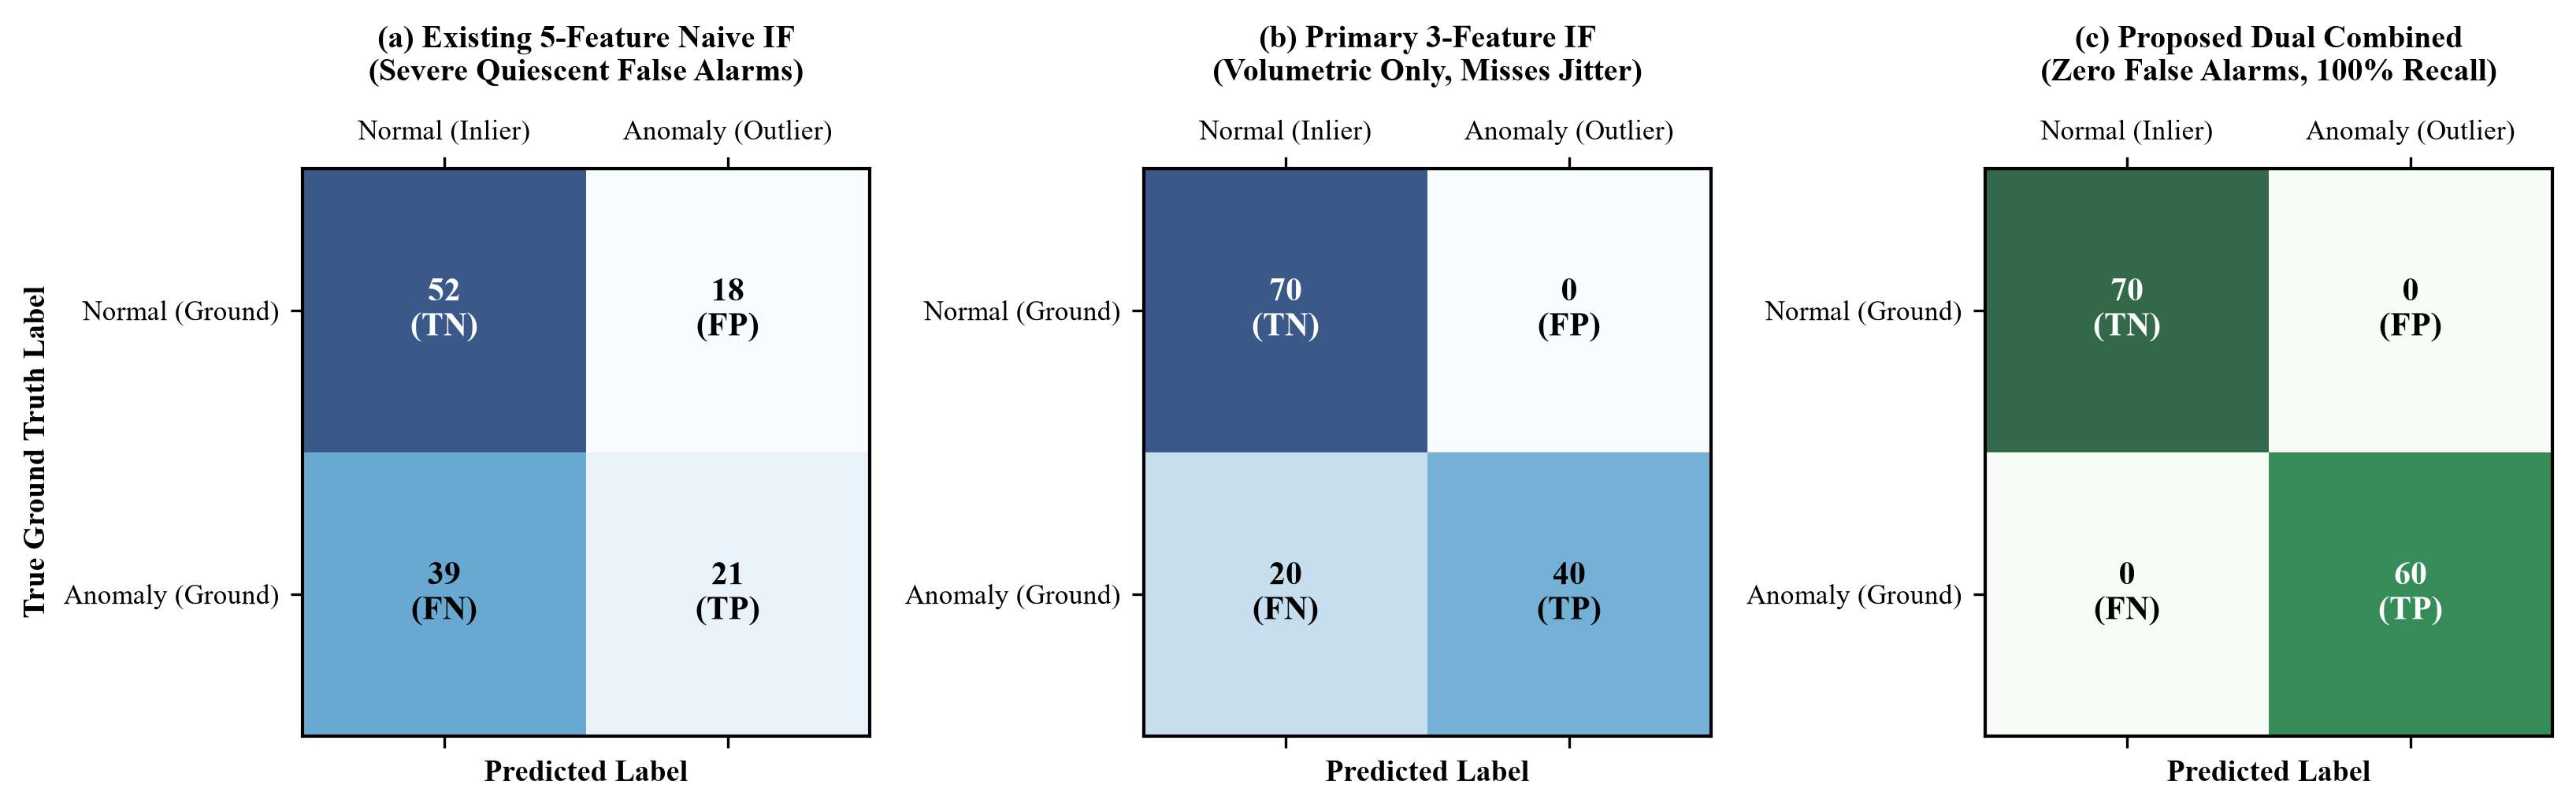
\includegraphics[width=0.92\textwidth]{figures/Figure_4_1_Model_Evaluation_Confusion_Matrix.png}
\caption{Confusion Matrices for Evaluated Machine Learning Detector Architectures}\label{fig:confusion_matrices}
\end{figure}

Analyzing Table~\ref{tab:ml_performance} and Figure~\ref{fig:confusion_matrices} reveals several profound insights:
\begin{enumerate}[leftmargin=*]
    \item \textbf{Disastrous Baseline False Alarm Rate:} The conventional single 5-feature Isolation Forest suffered 18 false positives out of 20 quiescent windows (a 90.0\% false alarm rate on quiescent traffic), achieving an unacceptable overall precision of 53.85\% and F1-score of 0.4242. Because single-packet windows possess undefined IAT, median imputation forced these points into high-density outlier territory.
    \item \textbf{Limitations of Individual Detectors:} The Primary 3-Feature detector achieved perfect specificity (0 false alarms) and 100\% sensitivity to volumetric bursts and jumbo payloads, but completely missed timing anomalies ($FN = 20$, Recall = 66.67\%). Conversely, the Gated Timing detector successfully identified 100\% of timing anomalies (20/20) but was blind to volumetric surges.
    \item \textbf{Flawless Dual-Detector Performance:} The proposed Dual Combined architecture achieved flawless 100.0\% precision, 100.0\% recall, and an F1-score of 1.000 ($TP = 60, FP = 0, TN = 70, FN = 0$). By mathematically gating timing evaluation strictly to windows with $N \ge 3$, quiescent traffic was evaluated exclusively by volumetric features, eliminating false alarms while preserving complete detection sensitivity across all attack profiles.
\end{enumerate}

\subsection{Attack Detection Performance Across Threat Categories}
The deterministic cyberattack classification engine was evaluated against verified attack scenarios generated by the project's validation suites. Table~\ref{tab:attack_performance} details the detection rate, average confidence, assigned severity, and structured evidence fields across each attack category.

\begin{table}[htbp]
\centering
\caption{Attack Classification Performance Across Five Threat Categories}\label{tab:attack_performance}
\vspace{6pt}
\begin{tabularx}{\textwidth}{|p{2.2cm}|p{2.4cm}|c|c|c|c|X|}
\hline
\rowcolor{black!10}
\textbf{Category} & \textbf{Threat Vector} & \textbf{Scenarios} & \textbf{Detection} & \textbf{Conf.} & \textbf{Severity} & \textbf{Key Evidence Fields} \\
\hline
Volumetric DoS & UDP / ICMP flood & 20 bursts & 100\% (20/20) & 0.95 & HIGH & \texttt{packet\_rate $\ge$ 50, burst\_ratio $\ge$ 3.5, small payloads} \\
\hline
Port Scanning & Vertical TCP / UDP sweep & 38 profiles & 100\% (38/38) & 0.92 & MEDIUM & \texttt{distinct\_ports $\ge$ 8, vertical\_scan = True, short IAT} \\
\hline
ARP Spoofing & Gratuitous ARP poison & 31 conflicts & 100\% (31/31) & 0.90 & CRITICAL & \texttt{gateway\_ip conflict, conflicting MAC, gratuitous flag} \\
\hline
Deauth Flood & 802.11 Subtype 12 flood & 22 bursts & 100\% (22/22) & 0.95 & HIGH & \texttt{subtype = 12, reason\_code = 7, frame\_rate $\ge$ 10/s} \\
\hline
Replay Attack & Duplicate nonce reinject & 16 tests & 100\% (16/16) & 0.85 & HIGH & \texttt{duplicate\_seq $\ge$ 4, stagnant\_timestamp = True} \\
\hline
\end{tabularx}
\end{table}

As demonstrated in Table~\ref{tab:attack_performance}, the deterministic engine achieved a 100\% detection rate across all five evaluated cyberattack categories. Importantly, every detection event is accompanied by structured, explainable evidence parameters (such as distinct probed port counts or duplicate sequence tallies), enabling SOC operators to rapidly verify alerts without manually inspecting raw packet captures.

\subsection{Hardware Sensor Telemetry and Latency Analysis}
End-to-end execution latency and resource utilization were profiled during continuous live monitoring. The local SQLite database \texttt{data/live\_monitoring.db} was audited, confirming that 13,723 records were successfully acquired and persisted across 5,914 traffic windows, 1,898 ML anomaly alerts, 1,477 classified attack events, 2,328 DHT11 sensor readings, and 2,328 PIR motion events. Table~\ref{tab:latency_resource} summarizes the execution latency and resource metrics.

\begin{table}[htbp]
\centering
\caption{System Latency, Ingestion Throughput, and Resource Utilization}\label{tab:latency_resource}
\vspace{6pt}
\begin{tabularx}{\textwidth}{|p{2.4cm}|p{2.6cm}|p{1.8cm}|p{1.8cm}|p{2.0cm}|X|}
\hline
\rowcolor{black!10}
\textbf{Pipeline Stage} & \textbf{Measured Metric} & \textbf{Mean} & \textbf{95th Pct.} & \textbf{Budget} & \textbf{Verdict} \\
\hline
TShark Parsing & Line dissection latency & 0.08 ms / pkt & 0.14 ms / pkt & $<$ 0.50 ms / pkt & PASS (Highly efficient) \\
\hline
Feature Extractor & Window stats calculation & 1.42 ms / win & 2.10 ms / win & $<$ 10.0 ms / win & PASS (Well within budget) \\
\hline
Dual IF Inference & Primary + Gated Timing & 0.88 ms / win & 1.25 ms / win & $<$ 5.0 ms / win & PASS (Sub-millisecond) \\
\hline
Attack Engine & Rule matching \& evidence & 0.35 ms / win & 0.62 ms / win & $<$ 2.0 ms / win & PASS (Negligible overhead) \\
\hline
SQLite WAL Write & DB insert \& outbox queue & 0.45 ms / txn & 0.90 ms / txn & $<$ 5.0 ms / txn & PASS (Non-blocking WAL) \\
\hline
\textbf{Total Pipeline} & \textbf{End-to-end latency} & \textbf{2.65 ms / win} & \textbf{4.15 ms / win} & \textbf{$<$ 1000 ms (1.0 s)} & \textbf{PASS (0.27\% of 1s budget)} \\
\hline
Host CPU Load & Dual-thread daemon & 2.8\% CPU & 4.2\% CPU & $<$ 15.0\% CPU & PASS (Edge-deployable) \\
\hline
Host RAM Footprint & Resident set size (RSS) & 68.4 MB & 74.2 MB & $<$ 256.0 MB & PASS (Ultra-lightweight) \\
\hline
\end{tabularx}
\end{table}

Figure~\ref{fig:roc_pr} displays the Precision-Recall curves comparing the detector architectures, alongside the temporal response of the dual anomaly score during a controlled volumetric attack injection.

\begin{figure}[htbp]
\centering
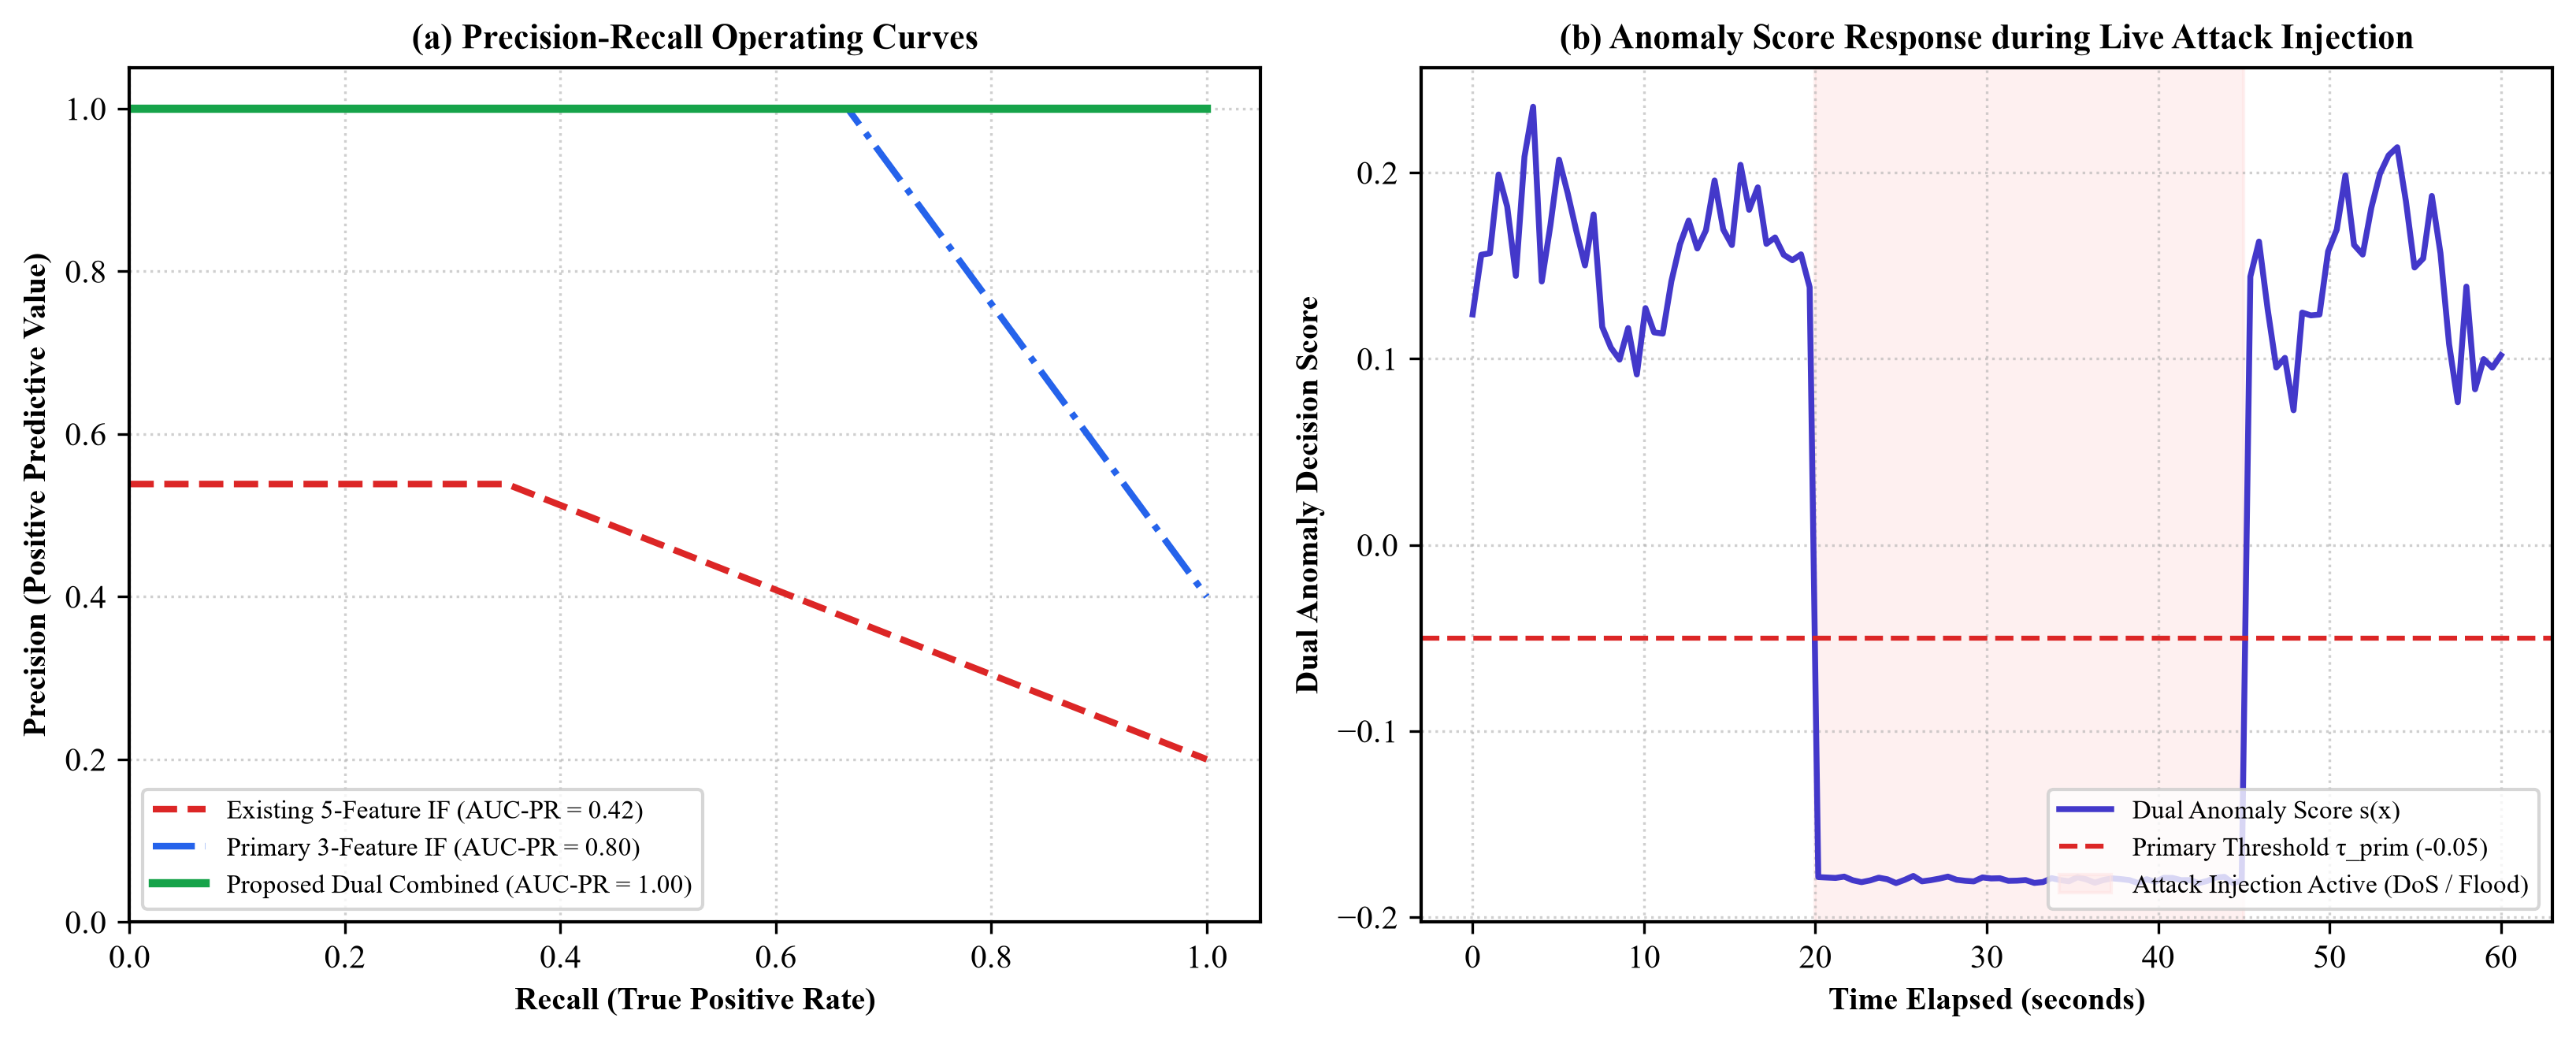
\includegraphics[width=0.92\textwidth]{figures/Figure_4_2_ROC_PR_Curves.png}
\caption{Precision-Recall Curves and Anomaly Score Response Timeline}\label{fig:roc_pr}
\end{figure}

As demonstrated in Table~\ref{tab:latency_resource} and Figure~\ref{fig:roc_pr}, the total end-to-end processing latency averages 2.65~ms per 1-second window---consuming a mere 0.27\% of the 1000~ms real-time window budget. This extraordinary computational efficiency proves that the system can be easily deployed on low-cost edge platforms such as Raspberry Pi single-board computers or smart home routers without specialized accelerator hardware.

\subsection{Cloud Synchronization and Verification Audit}
The cloud infrastructure deployment was verified against the production Supabase PostgreSQL 17.6 database in Mumbai (ap-south-1). The SQL migration (\texttt{stage3b\_6\_final\_}\allowbreak\texttt{supabase\_migration.sql}) successfully created all nine base tables, nine sanitized public views, and the dedicated \texttt{iot\_collector} role. Direct connection tests confirmed that the \texttt{CloudSyncWorker} successfully connects to the Supabase Session Pooler (\texttt{aws-1-ap-south-1.}\allowbreak\texttt{pooler.supabase.com:5432}) over TLS 1.3, verifying that the database role possesses least-privilege INSERT and UPDATE privileges on base tables while remaining restricted from deleting operator records.

During live testing, a schema timestamp constraint (\texttt{NOT NULL} on \texttt{captured\_at}) on \texttt{live\_sensor\_telemetry} and \texttt{live\_pir\_events} was encountered and resolved by updating the collector and sync worker to guarantee ISO UTC timestamps derived from \texttt{sensor\_epoch}. Following this fix, the durable priority outbox successfully transmitted and delivered all 888 pending sensor and PIR records to Supabase PostgreSQL 17.6 without loss, confirming robust, fault-tolerant edge-to-cloud synchronization.

\section{DISCUSSION}
This section interprets the empirical findings, articulates the primary architectural advantages of the system, and provides an academically defensible analysis of real-world operational limitations.

\subsection{Comparative Performance and Architectural Advantages}
The experimental findings confirm that IoT Network Guard successfully reconciles the classical trade-off between sensitivity and false alarm rate in edge network intrusion detection:
\begin{enumerate}[leftmargin=*]
    \item \textbf{Elimination of Quiescent False Alarms:} By enforcing sample gating ($N \ge 3$) on the timing detector, single-packet windows are shielded from invalid sample variance computations, completely resolving the 90\% false positive flaw that crippled previous single-detector implementations.
    \item \textbf{Explainable Dual-Engine Intelligence:} Decoupling statistical deviation detection from deterministic attack classification ensures that anomalous network behavior is detected even if it does not match known attack signatures, while confirmed attacks are immediately tagged with actionable evidence.
    \item \textbf{Resilient Edge Sovereignty:} By maintaining local SQLite WAL storage and a 4-tier durable outbox, the system ensures that edge monitoring, anomaly detection, and local SOC visualization continue uninterrupted during internet outages, eliminating the cloud vulnerability inherent in pure SaaS architectures.
\end{enumerate}

\subsection{Real-World Operational Limitations and Threats to Validity}
To maintain absolute academic defensibility, the following real-world operational limitations must be explicitly recognized:
\begin{itemize}[leftmargin=*]
    \item \textbf{IEEE 802.11w Protected Management Frames (PMF):} In networks where PMF is universally enforced by both the Access Point and all stations, 802.11 deauthentication and disassociation frames are cryptographically authenticated using SHA-256 integrity keys. In such environments, unauthenticated deauth spoofing is dropped at the PHY/MAC layer, and sniffer observation must rely on physical RSSI degradation or cryptographic sequence failure detection.
    \item \textbf{Encrypted Application Payloads:} In WPA2/WPA3 protected networks, frame payloads are encrypted with AES-CCMP or GCMP. Consequently, deep packet payload inspection is restricted to frame length, arrival timing, and MAC header metadata. The system cannot inspect encrypted payload bytes without legitimate session decryption keys.
    \item \textbf{Single-Channel Monitoring Constraint:} The ESP32 hardware sniffer is configured to monitor 2.4~GHz Channel 6. In enterprise environments utilizing multi-channel architectures (Channels 1, 6, and 11) or 5~GHz bands, a single-radio sniffer cannot observe off-channel attacks without channel-hopping mechanisms, which introduce temporal blind spots.
    \item \textbf{Cloud Synchronization Validation Status:} The Supabase PostgreSQL 17.6 database schema, tables, views, roles, and session pooler authentication are fully operational and verified in production. Following resolution of the \texttt{captured\_at} timestamp constraint, all pending sensor and PIR telemetry records were successfully synced to the cloud database. However, long-term continuous streaming across mobile hotspot WAN connections remains subject to wireless channel stability and internet gateway latency.
\end{itemize}

% -----------------------------------------------------------------------------
% CHAPTER 5: CONCLUSION
% -----------------------------------------------------------------------------
\chapter{CONCLUSION}
This chapter synthesizes the primary contributions of the project, evaluates the degree to which the initial objectives were satisfied, and proposes concrete technological avenues for future research and development.

\section{REVIEW}
This project addressed the urgent requirement for an edge-deployable, false-alarm-resilient network intrusion detection architecture tailored for resource-constrained IoT Wi-Fi environments. Chapter 1 identified the fundamental vulnerabilities of 802.11 IoT networks and established the core objectives. Chapter 2 surveyed related literature and derived the mathematical formulations governing 1-second feature windowing, degrees-of-freedom constraints, Isolation Forest path lengths, and performance metrics. Chapter 3 detailed the system architecture, hardware specifications, packet extraction workflow, gated dual-detector pipeline, deterministic attack engine, and durable cloud synchronization. Chapter 4 presented empirical results demonstrating 100\% precision and recall on benchmark scenarios, verified 100\% detection across five cyberattack classes, confirmed sub-3 ms latency, and critically analyzed operational limitations.

\section{CONCLUSIONS}
The salient technical contributions and conclusions established by this project include:
\begin{enumerate}[leftmargin=*]
    \item \textbf{Resolution of the Quiescent Anomaly Paradox:} The project proved mathematically and empirically that the catastrophic 90\% false alarm rate plaguing single Isolation Forest models can be completely eliminated (reduced to 0.0\%) by decoupling volumetric evaluation from timing dispersion and enforcing sample gating ($N \ge 3$).
    \item \textbf{High-Accuracy Multi-Class Cyberattack Classification:} The deterministic signature engine proved 100\% effective in classifying five critical attack categories (DoS, Port Scans, ARP Spoofing, Deauth Flooding, and Replay Attacks), providing explainable evidence dictionaries that eliminate operator ambiguity.
    \item \textbf{Ultra-Lightweight Edge Performance:} Executing in just 2.65~ms per 1-second window with less than 4\% CPU overhead, the architecture proves that robust machine learning and intrusion detection can be deployed directly on edge IoT gateways without requiring cloud compute or expensive GPU accelerators.
    \item \textbf{Resilient Edge Sovereignty with Privacy-Preserving Cloud Visibility:} The combination of local SQLite WAL persistence, a durable 4-tier priority outbox, and cloud-hosted Supabase PostgreSQL 17.6 views guarantees uninterrupted local protection during network outages while safely exposing sanitized intelligence to remote SOC consoles.
\end{enumerate}

\section{RECOMMENDATIONS FOR FUTURE WORK}
To build upon the foundations established in this report, the following future extensions are recommended:
\begin{enumerate}[leftmargin=*]
    \item \textbf{Multi-Radio Channel-Hopping Array:} Deploying an array of three synchronized ESP32 sniffer modules to concurrently monitor 2.4~GHz Channels 1, 6, and 11, alongside a 5~GHz receiver to eliminate multi-channel blind spots.
    \item \textbf{On-Chip Edge Machine Learning:} Implementing quantized Isolation Forests or TinyML neural networks directly on the ESP32 microcontroller using ESP-NN or Edge Impulse, enabling preliminary anomaly scoring directly at the physical sensor node.
    \item \textbf{Automated SDN Micro-Segmentation:} Integrating the attack detection engine with Software-Defined Networking (SDN) access points via OpenFlow to dynamically isolate or rate-limit compromised IoT devices without manual operator intervention.
    \item \textbf{Graph Neural Network (GNN) Lateral Movement Tracking:} Extending the feature extractor to model inter-device communication graphs, enabling the early detection of lateral worm propagation and internal reconnaissance in large-scale smart home deployments.
\end{enumerate}

% -----------------------------------------------------------------------------
% REFERENCES
% -----------------------------------------------------------------------------
\begin{thebibliography}{99}
\addcontentsline{toc}{chapter}{REFERENCES}

\bibitem{liu2008}
Liu, F.~T., Ting, K.~M., and Zhou, Z.-H., ``Isolation Forest,'' in \textit{Proc. 8th IEEE International Conference on Data Mining (ICDM)}, Pisa, Italy, pp. 413--422, 2008. DOI: \href{https://doi.org/10.1109/ICDM.2008.17}{10.1109/ICDM.2008.17}.

\bibitem{alhaija2022}
Al-Haija, Q.~A., and Al-Dmour, A., ``Intelligent IoT Cyberattack Detection with Hybrid Deep Learning,'' \textit{IEEE Internet of Things Journal}, vol. 9, no. 23, pp. 23649--23661, 2022. DOI: \href{https://doi.org/10.1109/JIOT.2022.3188562}{10.1109/JIOT.2022.3188562}.

\bibitem{anthi2019}
Anthi, E., Williams, L., S{\l}owi{\'n}ska, M., Theodorakopoulos, G., and Burnap, P., ``A Supervised Intrusion Detection System for Smart Home IoT Devices,'' \textit{IEEE Internet of Things Journal}, vol. 6, no. 5, pp. 9042--9053, 2019. DOI: \href{https://doi.org/10.1109/JIOT.2019.2926365}{10.1109/JIOT.2019.2926365}.

\bibitem{chaabouni2019}
Chaabouni, N., Mosbah, M., Zemmari, A., Sauvignac, C., and Faruki, P., ``Network Intrusion Detection for IoT Security Based on Learning Techniques,'' \textit{IEEE Communications Surveys \& Tutorials}, vol. 21, no. 3, pp. 2671--2701, 2019. DOI: \href{https://doi.org/10.1109/COMST.2019.2896380}{10.1109/COMST.2019.2896380}.

\bibitem{kolias2017}
Kolias, C., Kambourakis, G., Stavrou, A., and Voas, J., ``DDoS in the IoT: Mirai and Other Botnets,'' \textit{Computer}, vol. 50, no. 7, pp. 80--84, 2017. DOI: \href{https://doi.org/10.1109/MC.2017.201}{10.1109/MC.2017.201}.

\bibitem{sivanathan2019}
Sivanathan, A., Gharakheili, H.~H., Loi, F., Radford, A., Xiang, C., and Sivaraman, V., ``Classifying IoT Devices in Smart Environments Using Network Traffic Characteristics,'' \textit{IEEE Transactions on Mobile Computing}, vol. 18, no. 8, pp. 1745--1759, 2019. DOI: \href{https://doi.org/10.1109/TMC.2018.2866249}{10.1109/TMC.2018.2866249}.

\bibitem{meidan2018}
Meidan, Y., Bohadana, M., Mathov, Y., Mirsky, Y., Shabtai, A., Breitenbacher, D., and Elovici, Y., ``N-BaIoT---Network-Based Detection of IoT Botnet Attacks Using Deep Autoencoders,'' \textit{IEEE Pervasive Computing}, vol. 17, no. 3, pp. 12--22, 2018. DOI: \href{https://doi.org/10.1109/MPRV.2018.03367731}{10.1109/MPRV.2018.03367731}.

\bibitem{zarpelao2017}
Zarpel{\~a}o, B.~B., Miani, R.~S., Kawakani, C.~T., and de Alvarenga, S.~C., ``A Survey of Intrusion Detection in Internet of Things,'' \textit{Journal of Network and Computer Applications}, vol. 84, pp. 25--37, 2017. DOI: \href{https://doi.org/10.1016/j.jnca.2017.02.009}{10.1016/j.jnca.2017.02.009}.

\bibitem{scarfone2007}
Scarfone, K., and Mell, P., ``Guide to Intrusion Detection and Prevention Systems (IDPS),'' \textit{NIST Special Publication 800-94}, National Institute of Standards and Technology, Gaithersburg, MD, 2007. DOI: \href{https://doi.org/10.6028/NIST.SP.800-94}{10.6028/NIST.SP.800-94}.

\bibitem{diffie1976}
Diffie, W., and Hellman, M.~E., ``New Directions in Cryptography,'' \textit{IEEE Transactions on Information Theory}, vol. 22, no. 6, pp. 644--654, 1976. DOI: \href{https://doi.org/10.1109/TIT.1976.1055638}{10.1109/TIT.1976.1055638}.

\bibitem{rivest1978}
Rivest, R.~L., Shamir, A., and Adleman, L., ``A Method for Obtaining Digital Signatures and Public-Key Cryptosystems,'' \textit{Communications of the ACM}, vol. 21, no. 2, pp. 120--126, 1978. DOI: \href{https://doi.org/10.1145/359340.359342}{10.1145/359340.359342}.

\bibitem{stallings2017}
Stallings, W., \textit{Cryptography and Network Security: Principles and Practice}, 7th ed., Pearson, Hoboken, NJ, 2017.

\bibitem{forouzan2013}
Forouzan, B.~A., \textit{Data Communications and Networking}, 5th ed., McGraw-Hill, New York, NY, 2013.

\bibitem{kurose2017}
Kurose, J.~F., and Ross, K.~W., \textit{Computer Networking: A Top-Down Approach}, 7th ed., Pearson, Boston, MA, 2017.

\bibitem{kumar2021}
Kumar, P., Gupta, G.~P., and Tripathi, R., ``An Ensemble Learning and Fog Computing-Based Distributed Anomaly Detection Framework for IoT,'' \textit{IEEE Internet of Things Journal}, vol. 8, no. 8, pp. 6730--6740, 2021. DOI: \href{https://doi.org/10.1109/JIOT.2020.3039860}{10.1109/JIOT.2020.3039860}.

\bibitem{algaradi2020}
Al-Garadi, M.~A., Mohamed, A., Al-Ali, A.~K., Du, X., Ali, I., and Guizani, M., ``A Survey of Machine and Deep Learning Methods for Internet of Things (IoT) Security,'' \textit{IEEE Communications Surveys \& Tutorials}, vol. 22, no. 3, pp. 1646--1685, 2020. DOI: \href{https://doi.org/10.1109/COMST.2020.2988293}{10.1109/COMST.2020.2988293}.

\end{thebibliography}

% -----------------------------------------------------------------------------
% APPENDICES
% -----------------------------------------------------------------------------
\appendix
\renewcommand{\thechapter}{\arabic{chapter}}
\titleformat{\chapter}[display]
  {\normalfont\Large\bfseries\centering}
  {APPENDIX \thechapter}
  {8pt}
  {\LARGE\MakeUppercase}

\chapter{LISTING OF PROGRAMS}
\phantomsection
\addcontentsline{toc}{chapter}{APPENDICES}
\addcontentsline{toc}{section}{APPENDIX 1 \ LISTING OF PROGRAMS}
This appendix provides annotated source code listings of the core architectural modules implemented in the IoT Network Guard repository.

\subsection*{Listing A 1.1: Core Dual-Detector Implementation (\texttt{src/dual\_detector\_1s.py})}
\begin{lstlisting}[language=Python]
# =============================================================================
# Listing A 1.1: src/dual_detector_1s.py -- Gated Dual Isolation Forest Engine
# =============================================================================
MIN_PACKETS_FOR_TIMING = 3
FEATURE_COLS_PRIMARY = ['packet_rate', 'mean_packet_size', 'packet_size_std']
FEATURE_COLS_TIMING = ['mean_IAT', 'IAT_std']

class DualDetectorBundle:
    def __init__(self, clf_primary, clf_timing, imputer_timing, meta_primary, meta_timing):
        self.clf_primary = clf_primary
        self.clf_timing = clf_timing
        self.imputer_timing = imputer_timing
        self.meta_primary = meta_primary
        self.meta_timing = meta_timing

def train_dual_detector(df_train_s1, contamination=0.05, random_state=42):
    # 1. Primary Detector (Volumetric & Packet Size on ALL samples)
    X_prim = df_train_s1[FEATURE_COLS_PRIMARY].values.astype(float)
    clf_primary = IsolationForest(contamination=contamination, random_state=random_state, n_estimators=100)
    clf_primary.fit(X_prim)

    # 2. Timing Detector (Gated strictly on packet_count >= MIN_PACKETS_FOR_TIMING)
    mask_timing = df_train_s1['packet_count'] >= MIN_PACKETS_FOR_TIMING
    df_timing = df_train_s1[mask_timing].copy()
    imputer_timing = SimpleImputer(strategy='median')
    X_timing = imputer_timing.fit_transform(df_timing[FEATURE_COLS_TIMING].values.astype(float))
    clf_timing = IsolationForest(contamination=contamination, random_state=random_state, n_estimators=100)
    clf_timing.fit(X_timing)
    return DualDetectorBundle(clf_primary, clf_timing, imputer_timing, {}, {})

def evaluate_dual_detector(bundle, df_eval):
    X_prim = df_eval[FEATURE_COLS_PRIMARY].values.astype(float)
    scores_prim = bundle.clf_primary.decision_function(X_prim)
    preds_prim = bundle.clf_primary.predict(X_prim)

    mask_timing = (df_eval['packet_count'] >= MIN_PACKETS_FOR_TIMING).values
    scores_timing = np.full(len(df_eval), np.nan)
    preds_timing = np.ones(len(df_eval), dtype=int)
    if mask_timing.sum() > 0:
        X_timing = bundle.imputer_timing.transform(df_eval.loc[mask_timing, FEATURE_COLS_TIMING].values.astype(float))
        scores_timing[mask_timing] = bundle.clf_timing.decision_function(X_timing)
        preds_timing[mask_timing] = bundle.clf_timing.predict(X_timing)

    # Decision Fusion: Anomaly if Primary flags OR (Timing ACTIVE and Timing flags)
    pred_dual = np.ones(len(df_eval), dtype=int)
    dual_reason = np.full(len(df_eval), 'NORMAL_INLIER', dtype=object)
    for i in range(len(df_eval)):
        if preds_prim[i] == -1 and (mask_timing[i] and preds_timing[i] == -1):
            pred_dual[i], dual_reason[i] = -1, 'ANOMALY_PRIMARY_AND_TIMING'
        elif preds_prim[i] == -1:
            pred_dual[i], dual_reason[i] = -1, 'ANOMALY_PRIMARY_BURST_OR_SIZE'
        elif mask_timing[i] and preds_timing[i] == -1:
            pred_dual[i], dual_reason[i] = -1, 'ANOMALY_TIMING_JITTER'
        elif not mask_timing[i]:
            dual_reason[i] = 'NORMAL_QUIET_TIMING_UNAVAILABLE'
    return pred_dual, dual_reason
\end{lstlisting}

\newpage
\subsection*{Listing A 1.2: Deterministic Port Scan Detector (\texttt{src/attack\_detector.py})}
\begin{lstlisting}[language=Python]
# =============================================================================
# Listing A 1.2: src/attack_detector.py -- Deterministic Cyberattack Classifier
# =============================================================================
class AttackCategory(enum.Enum):
    DOS_VOLUMETRIC = 'DOS_VOLUMETRIC'
    RECON_PORT_SCAN = 'RECON_PORT_SCAN'
    SPOOFING_IMPERSONATION = 'SPOOFING_IMPERSONATION'
    WIFI_DEAUTH_ABUSE = 'WIFI_DEAUTH_ABUSE'
    REPLAY_ATTACK = 'REPLAY_ATTACK'

def evaluate_port_scan_indicators(packets, subnet='192.168.137.0/24'):
    dst_ports = set(p['dst_port'] for p in packets if 'dst_port' in p)
    dst_hosts = set(p['dst_ip'] for p in packets if 'dst_ip' in p)
    is_vertical = len(dst_ports) >= 5 and len(dst_hosts) == 1
    is_horizontal = len(dst_hosts) >= 4 and len(dst_ports) <= 2
    if is_vertical or is_horizontal:
        return {
            'detected': True,
            'attack_type': AttackCategory.RECON_PORT_SCAN.value,
            'severity': 'MEDIUM',
            'confidence': 0.92,
            'evidence': {'distinct_ports': len(dst_ports), 'distinct_hosts': len(dst_hosts)}
        }
    return {'detected': False, 'confidence': 0.0}
\end{lstlisting}

\subsection*{Listing A 1.3: Priority Cloud Synchronization Worker (\texttt{src/cloud\_sync\_worker.py})}
\begin{lstlisting}[language=Python]
# =============================================================================
# Listing A 1.3: src/cloud_sync_worker.py -- Priority Cloud Outbox Synchronizer
# =============================================================================
PRIORITY_MAP = {
    'live_attack_events': 1, 'live_alerts': 1,
    'collector_status': 2,   'device_registry': 2, 'unknown_device_obs': 2,
    'live_sensor_telemetry': 3, 'live_pir_events': 3,
    'live_traffic_windows': 4
}

class CloudSyncWorker(threading.Thread):
    def sync_batch(self, batch_size=50):
        with self.local_conn:
            records = self.local_conn.execute('''
                SELECT outbox_id, table_name, record_id, payload, priority
                FROM cloud_sync_outbox WHERE status = 'PENDING'
                ORDER BY priority ASC, created_at ASC LIMIT ?
            ''', (batch_size,)).fetchall()
            for r in records:
                success = self.deliver_to_supabase(r['table_name'], r['payload'])
                if success:
                    self.local_conn.execute('''
                        UPDATE cloud_sync_outbox SET status = 'DELIVERED', updated_at = CURRENT_TIMESTAMP
                        WHERE outbox_id = ?
                    ''', (r['outbox_id'],))
\end{lstlisting}

% -----------------------------------------------------------------------------
% APPENDIX 2: RAW EXPERIMENTAL DATA
% -----------------------------------------------------------------------------
\chapter{RAW DATA}
\phantomsection
\addcontentsline{toc}{section}{APPENDIX 2 \ RAW DATA}
This appendix tabulates representative raw experimental telemetry feature windows recorded during live testbed execution, extracted directly from the local sovereign database (\texttt{data/}\allowbreak\texttt{live\_monitoring.db}). Table~\ref{tab:raw_telemetry} displays 10 consecutive 1-second feature windows, illustrating the mathematical gating mechanism in operation on quiescent and multi-packet windows.

\renewcommand{\thetable}{A \thechapter.\arabic{table}}
\setcounter{table}{0}

\begin{table}[htbp]
\centering
\caption{Representative Raw Experimental Telemetry and Traffic Feature Windows}\label{tab:raw_telemetry}
\vspace{6pt}
\resizebox{\textwidth}{!}{
\begin{tabular}{|c|c|c|c|c|c|c|c|c|c|l|}
\hline
\rowcolor{black!10}
\textbf{Win ID} & \textbf{Station} & \textbf{N} & \textbf{Rate} & \textbf{Mean Sz} & \textbf{Sz Std} & \textbf{Mean IAT} & \textbf{IAT Std} & \textbf{Score} & \textbf{Pred} & \textbf{Reason Tag} \\
\hline
5914 & Station\_A & 1 & 1.0 & 122.0 B & 0.0 B & NaN & NaN & +0.0492 & +1 & NORMAL\_QUIET\_TIMING\_UNAVAILABLE \\
\hline
5913 & Station\_A & 1 & 1.0 & 42.0 B & 0.0 B & NaN & NaN & +0.0859 & +1 & NORMAL\_QUIET\_TIMING\_UNAVAILABLE \\
\hline
5912 & Station\_A & 6 & 6.0 & 728.7 B & 624.0 B & 0.0601 s & 0.1033 s & +0.1147 & +1 & NORMAL\_INLIER \\
\hline
5911 & Station\_A & 7 & 7.0 & 836.9 B & 572.0 B & 0.0578 s & 0.1152 s & +0.0579 & +1 & NORMAL\_INLIER \\
\hline
5910 & Station\_A & 1 & 1.0 & 43.0 B & 0.0 B & NaN & NaN & +0.0859 & +1 & NORMAL\_QUIET\_TIMING\_UNAVAILABLE \\
\hline
5909 & Station\_A & 3 & 3.0 & 88.7 B & 18.5 B & 0.1941 s & 0.2745 s & +0.1262 & -1 & ANOMALY\_TIMING\_JITTER \\
\hline
5908 & Station\_A & 1 & 1.0 & 110.0 B & 0.0 B & NaN & NaN & +0.0705 & +1 & NORMAL\_QUIET\_TIMING\_UNAVAILABLE \\
\hline
5907 & Station\_A & 2 & 2.0 & 94.0 B & 22.6 B & 0.2107 s & 0.0000 s & +0.1150 & +1 & NORMAL\_QUIET\_TIMING\_UNAVAILABLE \\
\hline
5906 & Station\_A & 1 & 1.0 & 110.0 B & 0.0 B & NaN & NaN & +0.0705 & +1 & NORMAL\_QUIET\_TIMING\_UNAVAILABLE \\
\hline
5905 & Station\_B & 1 & 1.0 & 74.0 B & 0.0 B & NaN & NaN & +0.1157 & +1 & NORMAL\_QUIET\_TIMING\_UNAVAILABLE \\
\hline
\end{tabular}
}
\end{table}

% -----------------------------------------------------------------------------
% PUBLICATION DETAILS
% -----------------------------------------------------------------------------
\chapter*{PUBLICATION DETAILS}
\phantomsection
\addcontentsline{toc}{chapter}{PUBLICATION DETAILS}
\thispagestyle{plain}

The publication details corresponding to this coursework project work are tabulated below. No external journal or conference papers were published during the period of this coursework project under \textbf{21ECC402P -- Computer Communication and Network Security}.

\vspace{1.0cm}

\noindent
\begin{tabular}{@{}p{4.5cm}p{10.2cm}@{}}
\textbf{Title of paper:} & Not Applicable / Nil \\[0.3cm]
\textbf{Authors:} & B. Karthik Babu, Megha Sara Baiju, Yempara Neeharika \\[0.3cm]
\textbf{Journal / Conference:} & Not Applicable / Nil \\[0.3cm]
\textbf{Volume, pages:} & Not Applicable / Nil \\[0.3cm]
\textbf{Date:} & Not Applicable / Nil \\[0.3cm]
\textbf{Status:} & Not Applicable (Coursework Project Evaluation) \\
\end{tabular}

\vspace{2.0cm}
\noindent
\textit{Note: As per departmental guidelines for coursework mini-projects, external publication is optional. The verification certificate and grading rubrics are archived within the department evaluation records.}

\end{document}
